\documentclass[a4paper]{article}
%\documentclass[a4paper,sfsidenotes]{tufte-book}
\usepackage{localstyle} % local style file

% Oh for some fun!
%\usepackage{mathspec}
%\setmainfont{PragmataPro}
%\setmonofont{PragmataPro}
%\setmathfont(Digits,Latin,Greek)[StylisticSet=3]{PragmataPro} % Fraktur math!
%\setsansfont{PragmataPro}

\title{Using Authorization Logics To Make Decisions in Mobile Systems\\\vspace{2em}Thesis Proposal}
%\title{Security Policies\\For Humans\\Thesis Proposal}
\author{Joseph~Hallett}
\date\today

\hypersetup{%
  pdftitle={Thesis Proposal},
  pdfauthor={Joseph Hallett},
  hidelinks
}

\bibliographystyle{plainnat}
\begin{document}
\maketitle
\setcounter{tocdepth}{3}
\tableofcontents
\pagebreak

\section{Introduction}

Android is an operating system for mobile phones.  Users run prepackaged
software (\emph{apps}) which they download from special app stores.

\begin{marginfigure}
  \includegraphics[width=\marginlength]{img/facebookperms.jpeg}
  \caption{Some of the permissions requested by the Facebook app on Android.
  When installing an app a user is presented with a list of permissions the app
requires to run.  Permissions describe what phone features an app will have
access to.}
  \label{fig:fb}
\end{marginfigure}

When an app is installed on Android the user is prompted to accept the
privileges required by the app.  The user makes a decision based on what they
know about the app and their own personal security policies.  Most users accept
the app without thinking about it~\cite{Felt:2012hm}.  They do this for a many
reasons: because they don't understand the risks, they don't understand the
permissions, or they simply don't care and will install the app whatever.

Facebook is an example of an app which requests a large number of permissions
(Figure~\ref{fig:fb}). Users trust Facebook not to be malicious even though it
has access to amount of their personal data.  Some apps are over
privileged~\cite{Felt:2011kj}: they request permissions that grants them access
to data they do not use. Some apps are malicious~\cite{Zhou:2012cf}: they
request permissions to steal data or to spend money without the users consent.
Other apps are \emph{\ac{PUS}}\footnote{Whilst Google favor the term \ac{PUS} to
describe this kind of malware other names are also used. PUA (potentially
unwanted applications) and PUP (potentially unwanted programs) are other names
for the same family of malware.  These terms can be used interchangeably.}:
these are apps which are generally not malicious but may have features that goes
against what the user wants.  On a PC this might be a browser tool bar bundled
with another program.  On Android \ac{PUS} might be an aggressive advertising
framework that leaks private information or repeatedly polls GPS information
draining the phones battery~\cite{Svajcer:2013tp}.

More generally users and computers make decisions. Whether it is to update an
app or to connect to a website: the decisions are made based on the security
policies and trust relationships of the user and device.  These security
policies may include the use of tools or experts to decide whether something is
malicious.  For instance a user may trust a firewall program to enforce their
network policy; and they may trust a tool like
\emph{Shorewall}~\cite{Shorewall:uh,Tongaonkar:2007ua} to write
policy for them.  Alternately a user might wish to be able to install apps but
only trust apps \emph{Amazon} have vetted to be installed on their device.
\emph{Broadly, the aim of this research is to formalize these security policies
so they can be studied precisely and enforced automatically.}

Mobile operating systems are similar to existing systems but have a
different trust model and are used differently.  Software is
bought and downloaded from app stores, Apps run within sandboxes and collaborate
to share data. The devices contain more personal data
than before: sensors tracking users' locations,  gyroscopes measuring how
users move, and microphones listening to users calls.  The \ac{BYOD} trend
encourages users to take the devices they have at home into work.
This creates a tension between how the corporate IT department may require
employees to use their devices and the user's policies on how they want to use
their devices.  These features add a novel challenge to modelling these devices
and the stores and users surrounding them.  

Formalizing policies allows comparisons to be made between different systems and
the user's policies.  Common comparisons the two biggest mobile OSs, iOS and
Android, are informal: iOS is closed, more of a \emph{walled garden}. Apps go
through a vigorous review process and Apple is selective about what it sells.
Android is more permissive.  With a formal language to describe system policy we
can make a precise comparison. 

To analyze permissions, detect malware, static analysis has been used.
Static analysis tools infer (and occasionally enforce) complex security
properties about the code.  What is missing is the link between the assurances
these tools can give and the \emph{user-level policies} we want to enforce.  A
user-level policy describes how a user wishes an app to behave; though a user
may only specify them informally.

By using an \emph{authorization logic} as the glue layer we can enforce the
policy by building on the work on access control in distributed systems.  Static
analysis tools can be trusted to give statements about code, as can other
analysts and principals, that can be combined to implement a security policy.

This thesis research will show how authorization logics can be used to make
security decisions in mobile devices.  Security decisions are made manually by
smart phone users and it is our belief that by automating these choices users
can avoid having to make security decisions and their overall security be
improved.  To do this we plan: 

\begin{itemize}
  \item \emph{To model the decisions and trust relationships inherent in Android
    and other mobile operating systems.}  We will write security policies that
    describes the current state in these systems and serve as a base to compare
    systems. 

  \item \emph{To instantiate a logic of authorization that allows us to model
    the trust relationships between the components of an operating system and
  the users.}  This will include using static (and dynamic) analysis tools to
  make decisions.  These tools will be introduced as \emph{principals}: entities
  which say things about others.  The logic will be able to model what happens
  when apps can collude.  The logic will be based on earlier work on the
  \emph{SecPAL~language}~\cite{Becker:2006vh} that has been used for distributed
  access control decisions.

  \item \emph{To implement an app store that serves users only the apps that
    meet their security policies.}  This will include a user-study where we
    evaluate how well users comprehend their policies and the decisions made for
    them. This may lead into generating proof-carrying code
    certificates~\cite{Necula:1996tr} for apps that allow a device to check that
    their policy was met without having to do the full inference themselves.

  \item \emph{To study how users understand their security policies and the ways
    these policies are enforced.}   SecPAL is claimed to be more readable
    compared to other authorization logics and access control
    languages\cite{Gurevich:2008fz}.  Whilst end-users may not want to write
    their own policies system administrators and expert users should be able to
    comprehend what a policy means; they should understand why their policy
    allows some decisions and not others.

  \item \emph{To explore how security policies change with time and when apps
      can collude.}  A user's security policy need not be static.  People change
    jobs and may bring old devices to new environments requiring new security
    policies.  Apps can collude: two apps might meet a security policy when
    considered on their own but together they might act to share data
    inappropriately.  Over time an app might want greater access and increased
    permissions to support new functionality.  If this increased functionality
    breaks policy what should happen?  What should happen when a policy changes
    on a device or is revoked entirely?  It is not obvious how to write
    and check security policies for these scenarios; or how
    to enforce the policy at runtime.

\end{itemize}

\subsection{A Logic of Authorization For Mobile Devices}

Logics of authorization are used to decide whether someone may do something.
This might be carrying out an action, accessing data, or describing what another
entity can do. When we apply these logics to files and information we create an
access control system. A review of the history and applications of
the logics is given later in this proposal (page~\pageref{sec:pollang}); but in
summary they have shown themselves to be useful for modelling the
complex security and trust policies in modern systems.

Mobile devices are different to traditional computers. They have more
information about their users. They don't offer the user the traditional file
system interfaces. Everything is sandboxed and closed software markets (app
stores) distribute software.  The app stores typically allow developers to sell
their apps but are selective about what they will sell.  Apps are vetted for
quality and security\footnote{We believe: very few stores document their
  policies.  The \emph{Firefox Marketplace} is a notable exception as they
  publish their review criteria online:
  \url{https://developer.mozilla.org/en-US/Marketplace/Submission/Marketplace_review_criteria}.
Apple do publish a long list of guidelines as to what will be accepted or not,
but it is not exhaustive and does not state how they check:
\url{https://developer.apple.com/appstore/resources/approval/guidelines.html}. }.
  Static and dynamic analysis tools are used as well as traditional inspection.
  The policies the app stores apply to their apps form an authorization decision
  (\emph{the analysis team says app can be sold}) and there is a delegation of
  trust to the analysts and their tools. It is not clear how these policies and
  trust relations filter through to the end users.

These differences amount to a different model of trust than traditional machines
such as PCs and embedded systems. There are a new set of authorization problems
that are not obvious how to express in some authorization logics.  One problem
is how an app store should convince a device an app meets its policy; if
checking a policy cannot be done on a phone (maybe the battery is running low)
can checking be delayed?  What happens when two trusted principals disagree (as
might happen with apps in different stores)?  Some languages, like
Cassandra\cite{Becker:2004fi}, authorize on the basis of the speaker holding a
role; but what are the roles when a store has a changing policy?  

To solve these problems we have taken an existing authorization logic,
SecPAL~\cite{Becker:2006vh}, and extended it with a series of predicates that can
describe how security policies are met inside a mobile ecosystem.  Future work
will include describing the current security policies for Android and other
mobile OSs as well as the app acceptance policy for some app stores.  This will allow comparisons to be
made between them, and (with a database of apps) comparing what kinds of apps
different markets allow.

\subsection{Compound Policies Over Time}\label{sec:polovertime}

Consider a user who has a smart phone and is buying apps.  The
user must decide if they want to install an app: to do this they apply a series
of judgements called their \emph{security policy}.  

\begin{marginfigure}
  \label{fig:policies}
  \includegraphics[width=\marginlength]{img/policies.eps}
  \caption{Different policies being applied to one another.  Users, businesses
  and stores are all subject to regional laws.  A store may have a policy but
the developers who write the apps may also add their own rules in.  Devices
might have their own policies set by their designers but also have the OS
policies.  If the device is used on a network certain traffic may be restricted.
The user's policy (in red) is just one component of this ecosystem and cannot be
considered on its own.}
\end{marginfigure}

The user has their own security policy. They also have other security policies
they implicitly follow.  When they download apps from an app store they also
gain the security policy of the store and what it will sell.  If the phone runs
in a corporate environment then they may also be subject to the company's
corporate policy.  The operating system itself may have certain restrictions on
what it will allow.  The APK app format used on Android can also be installed on
Blackberry and Sailfish operating systems.  Each system may add
additional restrictions that may make some apps not installable.  An example of
how a compositional policy might be written is shown in
Figure~\ref{example:composition}.

\begin{marginfigure}\label{example:composition}
  \begin{lstlisting}[language=SecPAL]
Phone says app is-installable
  if app meets UserSecurityPolicy,
     app meets AppStorePolicy,
     app meets ITDeptPolicy,
     app meets OSPolicy.

Phone says User can-say inf
  app meets UserSecurityPolicy.

Phone says PlayStore can-say 0
  app meets AppStorePolicy.

Phone says ITAdmin can-say inf
  app meets ITDeptPolicy.
  \end{lstlisting}
  \caption{A compound security policy where an installation policy for a
    phone is dependent on other security policies.}
\end{marginfigure}
     
Suppose the phone uses this policy for a while but the user changes jobs.
Now they have to meet a new \code{ITDeptPolicy} set by a different administrator.
Should any installed apps be uninstalled if they don't meet the new policy?  If
we already have a certificate showing the apps passed the old policy can we
reuse it to create a new certificate that shows the app meets any additional
restrictions? 

What about the data an old version of an app may have stored?  If
an app were to reduce its permissions but still have access to the data then
there is a risk of an information leak.  Simply deleting the old data isn't good
enough as a user may still need their documents.

Whilst other authorization logics have looked at making one-time decisions about
whether to allow a computer to make a decision; there has been less work on
modelling these policies over time and seeing how a changing security policy
affects a changing device.

Alternatively say there is an app which the developer is continually improving
and adding new features.  When the app is installed it may meet the security
policy but with increasing features requiring access to more permissions and
introducing more complexity or a change of advert library the app no longer
meets the security policy.

Should the app be removed?  If the app is used every day by then the user may
not be pleased that the phone has decided to break their favorite
app; regardless of whether the fault lies with app developer or the policy
designer. Equally just stopping updates for the app increases app
version fragmentation and reduces security by rejecting bug fixes.  Allowing the
update isn't correct either as it means breaking the security policy.

Whilst there have been several papers looking at (and proposing methods to stop)
excessive permissions in applications~\cite{Felt:2011kj,Vidas:2011wr} there
has not been a thorough review of how permissions change for apps over time
and between versions of the same app as far as we know. 

% TODO ADD BIT EXPLAINING HOW TO DO THIS


\subsection{Personally Curated App Stores}

Apps are normally distributed on mobile devices through an app
store.  On iOS users have the \emph{App Store}: a curated market place run by
Apple (though other, albeit clunkier, distribution mechanisms do exist such as
the \emph{\ac{OTA}} update mechanism used for testing and some apps banned from
the App Store\footnote{An example of this would be the \emph{GBA4iOS} emulator:
(\url{http://gba4ios.angelxwind.net/download/}.  Emulator apps are seen to
support video game piracy so Apple does not allow them to be sold in the App
Store.}) that is perceived as being picky about the apps it sells.

Android users have a far greater choice of marketplace.  The \emph{Play Store}
is the app store distributed by Google. It is less moderated than Apple's store.
Amazon have their own app store that serves as a more curated version of
Google's offering. It is the default on their Kindle tablets.  Other app stores
target specific regions: such as \emph{Anzhi} and \emph{gFan} in China, or the \emph{SK~T-Store}
in Korea.  Some, such as \emph{Yandex.Store, AppsLib and SlideMe}, are
pre-installed by OEMS who can't or don't want to meet Google's requirements for
the PlayStore.  The \emph{F-Droid} store only delivers open source apps. Others
exist to distribute pirated apps. 

\begin{figure*}\centering\footnotesize
  \begin{tabular}{l l l p{0.1\linewidth} p{0.15\linewidth} p{0.25\linewidth}}
    \toprule
    Store & Region & Apps & Downloads (per month) & Security & Notes \\
    \midrule
    PlayStore & Worldwide & $800\times10^6$ & $2.5\times10^9$ & Estimated $0.01\%$ malware (F-Secure labs) & The default app store for Android devices.\\
    \addlinespace \\
    Yandex.Store & Russia & $50\times10^3$ & & Anti-virus scanning provided by Kaspersky. & Pre-installed by six OEMs. Used as the Android-app app store on the Jolla operating system. \\
    \addlinespace \\
    Anzhi & China & $180\times10^6$ & $2.2\times10^3$ & Estimated $5\%$ malware (F-Secure labs) & Quarter of a million users.\\
    \addlinespace \\
    SK-T Store & Korea & $70\times10^6$ & $28\times10^6$ & & \\
    \addlinespace \\
    SlideME & Worldwide & $40\times10^3$ & $15\times10^3$ & Using multiple malware scanners including one by \emph{BlueBox security} that can detect apps exploiting the master key vulnerability. & Installed by 140 OEMs. Twenty million users. \\
    \addlinespace \\
    Amazon AppStore & Worldwide & $76\times10^3$ & $25\times10^6$ & & Used on
    Kindle tablets, but popular on Android. \\
    \bottomrule
    \\
  \end{tabular}
  \caption{Summary of different app stores available for Android using data
    taken from the \emph{One Platform Foundation} list of App Stores:
    \texttt{http://www.onepf.org/appstores/}.}
    \label{tab:stores}
  \end{figure*}

On average eight percent~\cite{AQUILINO:2013wr} of the apps in each of these
alternative market places is malware. The Play Store contains very little
malware however (0.1\% of total apps), whilst a third of the app in the
Android159 store were found to be malicious.

Every app store has a different security policy.  They enforce these
policies when they pick which apps to sell to their users.  By using an
authorization logic to decide whether apps will meet a security policy we have
the ability to create a new kind of app store where offerings are tailored to
the user's security policy.  By creating app stores tailored to a security
policy we also give ourselves a way to empirically measure how restrictive a
security policy is: we can measure the number of apps offered inside the stores.

To enhance trust in the store digital evidence could be offered
with the apps This would give devices a practical means to check the app is
supported by their security policy without having to re-run all the static
analysis checks
themselves. This should also save device battery life.  

Proof-carrying authentication~\cite{Appel:1999dq} and authorization logics such
as BLF~\cite{Whitehead:2004bu} have already introduced ideas from proof-carrying
code into authorization logics. The focus of their work has been on
access control where a user is providing a proof that they have the credentials
to access a resource.   In the scenario we propose the role of the user is
reversed: the store offers many proofs to the user to increase their trust in
its wares; rather than the user offering one specific proof to prove they have
the right to complete a certain action.


\subsection{Project Context (App Guarden)}

\begin{figure}
  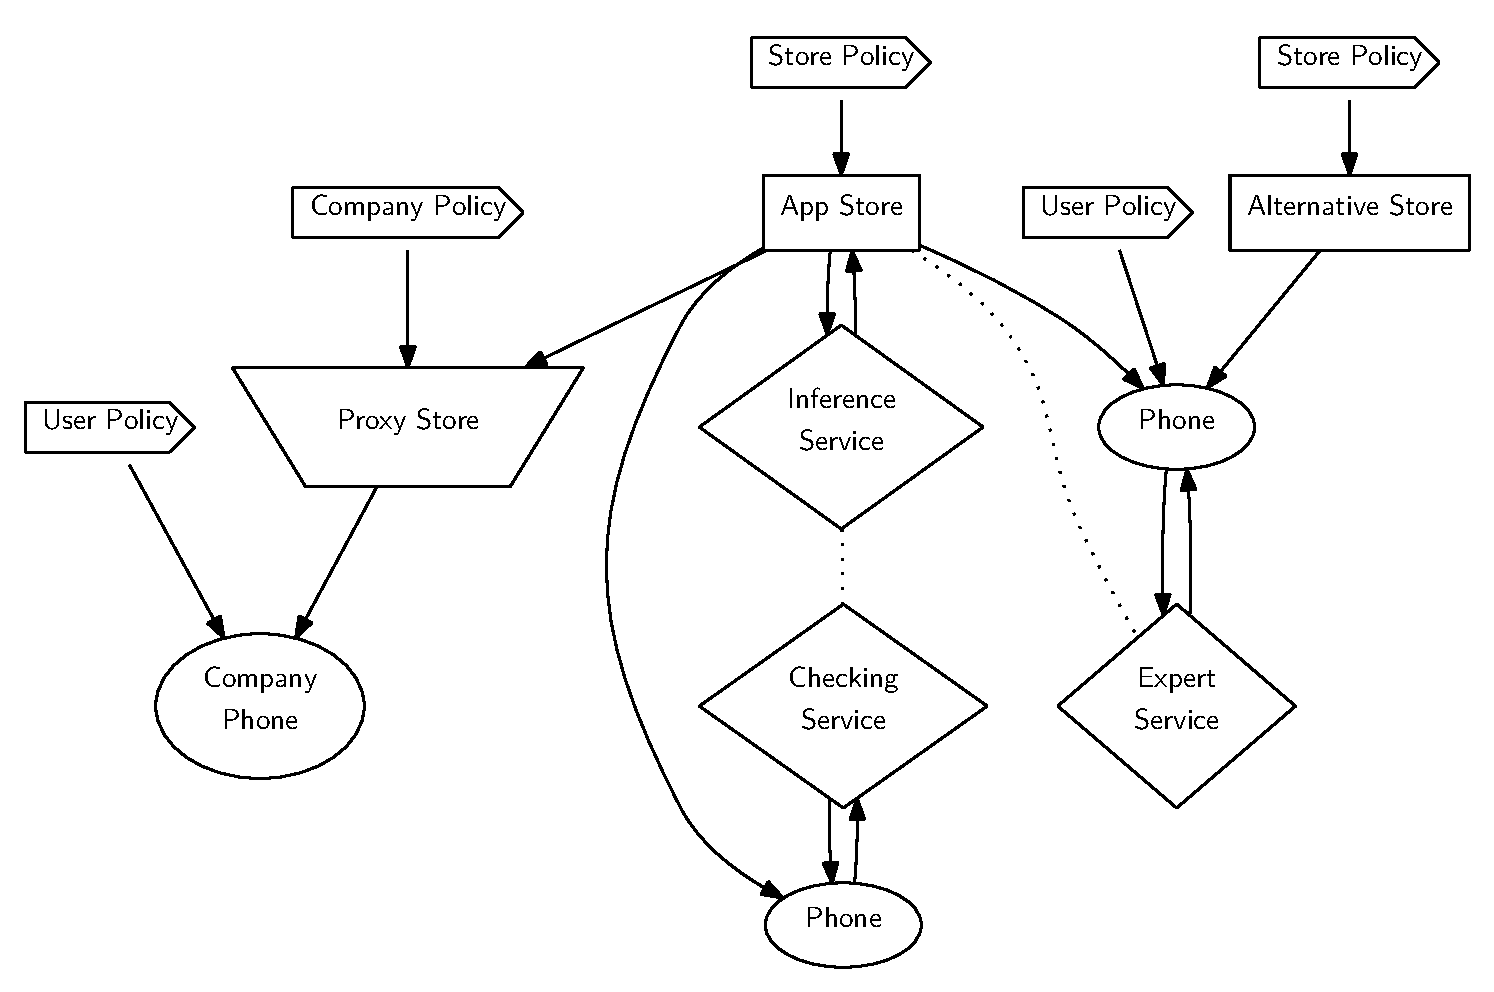
\includegraphics[width=\linewidth]{img/appguarden.eps}
  \caption{Overview of the different entities in App Guarden.  Each of the ovals
  represents a different device inside the system; each rectangle or trapezium
  represents  different supplier of apps, and each diamond is an authority that
  makes statements about apps and other software decisions.  Arrow boxes show
policies.  Arrows represent transfers of information or apps, and dotted line
indicate that the two entities are connected in some other way.}\label{fig:ag}
\end{figure}

This thesis will form part of the \emph{App
Guarden}\footnote{\url{http://groups.inf.ed.ac.uk/security/appguarden/Overview.html}}
project.  The App Guarden project aims to improve the quality of mobile security
by developing new tools to analyze apps and the app stores that sell them.

This work contributes by developing the security policies that describe what the
user wants and showing how they can be enforced using the tools that can check
security policies within the code.  The end result might be a system as shown in
Figure~\ref{fig:ag} where devices are interacting with stores and security
services such as static analysis tools or proof checkers. 

\begin{marginfigure}
  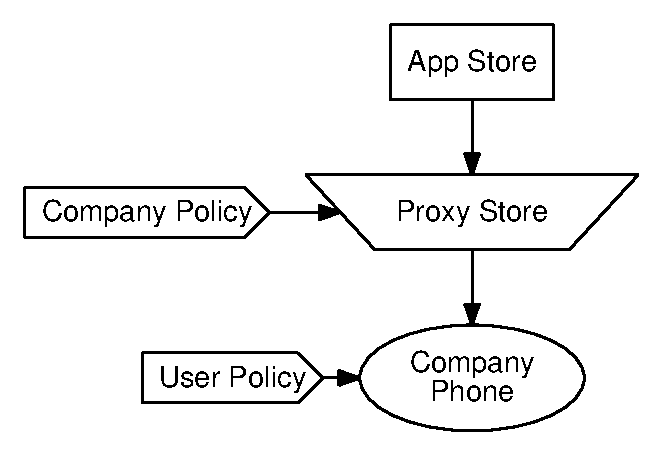
\includegraphics[width=\marginlength]{img/proxystore.eps}
  \caption{Security policies and the proxying store}
  \label{fig:proxy}
\end{marginfigure}

\begin{marginfigure}
  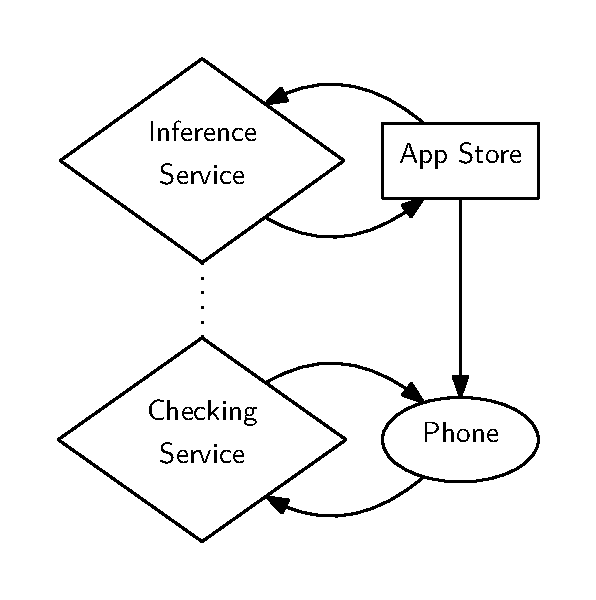
\includegraphics[width=\marginlength]{img/digitalevidence.eps}
  \caption{Checking services and an app store.}
  \label{fig:de}
\end{marginfigure}

\begin{marginfigure}
  
  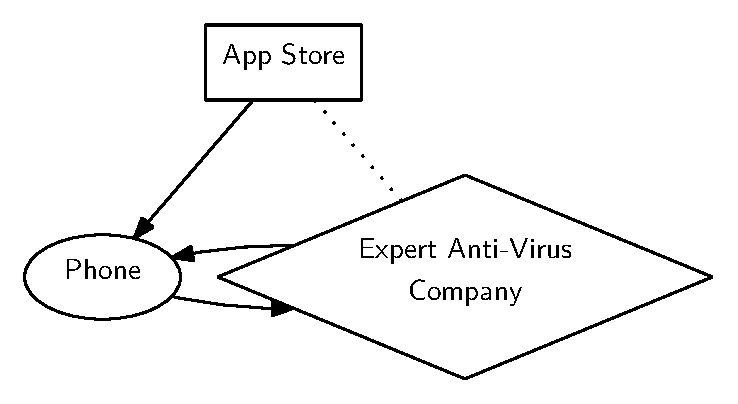
\includegraphics[width=\marginlength]{img/mcafee.eps}
  \caption{Use of an expert checker.}
\label{fig:mcafee}
\end{marginfigure}

\begin{marginfigure}
  
  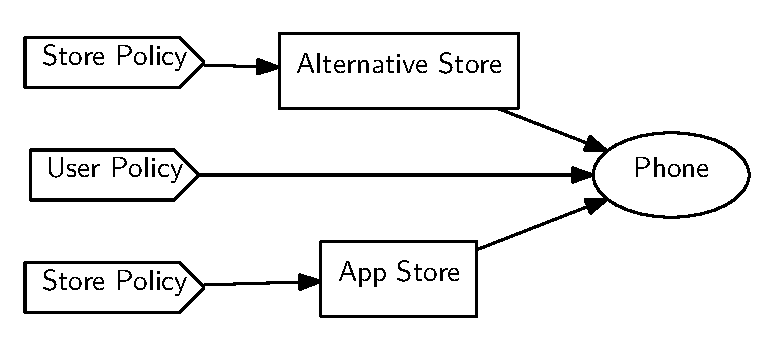
\includegraphics[width=\marginlength]{img/altstore.eps}
  \caption{A device using multiple stores with different policies.}
\label{fig:altstore}
\end{marginfigure}

Between each of the nodes different policies could be enforced.  Consider an
\emph{app store} and \emph{proxy store}.  There is a master app store that sells
many apps.  A company provides its employees each with a phone that they can
install apps on but they have their own security and usage policy set by their
IT department.  Employees shouldn't install anything that breaks the policy. On
all the devices the IT department provide they install a special proxy app
store.  The proxy app store takes apps from the main store but discards any apps
which might break the policy it is supplied with.  Users may download apps from
the company store, but they might exercise their own judgement and only download
apps that meet their own policies.  At each stage (as shown in
Figure~\ref{fig:proxy}) judgements are being made about what is acceptable from
an app store, and the policies are refined.

Another example might be an app store that supplies apps with \emph{digital
evidence}.  When the app store sells an app it wants to reassure its users that
it real guarantees that the app it is selling meets the security guarantees it
claims.  Being able to infer these properties is complex and takes both time and
battery power; this is difficult as many phones are battery constrained.  To
avoid this the app store uses an inference service to produce digital evidence
to be supplied with the app that shows (with the aid of a checking service that
could be running on the device) that an app meets the policy (as shown in
Figure~\ref{fig:de}). Other parts of the App Guarden project are 
developing these tools.

An alternative form of this could be where a store delegates to an expert third
party to make statements about the apps it sells.  One might imagine a scenario
where an app store might claim \emph{``We don't sell viruses in our store, but
don't take our word for it: here's a well known anti-virus company that will
verify our claim''} (as shown in Figure~\ref{fig:mcafee}).

If a user is using multiple stores (for example a jail broken iPhone user might
buy apps from both the App Store and the Cydia Store) then the policies the user
might be applying become complex (as described in Figure~\ref{fig:altstore}).
This leads to interesting questions around how policies should be composed and
the equivalence of security policies when they are; as well as questions about
the overall device policy in a system.

The work for this thesis will not concern itself with the development of tools
to check the apps perform as they should; rather it will focus on modeling the
trust relationships between these tools and the other entities in a mobile
environment.  This allows this part of the work to focus on the relationships
and device policies rather than the intricacies of code analysis.


\section{Review of Android Security}

Android is a Linux OS for mobile phones and consumer electronics. It has a large
software market of apps. Apps on the Dalvik virtual machine.  Dalvik is a
modified JVM architecture: it uses registers rather than stacks to save memory
and reduce code size; and drops some type information (again for space).  Apps
use a sandbox provided by the OS that is based on Linux's permissions
model~\cite{Drake:2014uq}.

\subsection{Permissions and Apps}

\begin{marginfigure}
  \centering
  \includegraphics[width=\marginlength]{img/brightestflashlight.png}
  \caption{The \emph{Brightest Flashlight Free} app prompting for its permissions
    at install time. This app is over privileged as a flashlight app should have
    no need for GPS or phone data, or network access.  This extra functionality
  was used maliciously.}
\label{img:brightestflashlight}
\end{marginfigure}

Android permissions come in three varieties: API permissions, file system
permissions, and IPC permissions.  API permissions say what high level
functionality an app may access.  For example the \texttt{INTERNET} permission
allows apps to access the network.  To enforce this Android uses the
Linux file system permissions in the underlying operating system: the
\texttt{/etc/permissions/platform.xml} file defines mapping between the API
and file system permissions.  In this case any process started from an app with
the \texttt{INTERNET} is assigned the \texttt{inet} file system permission which
is used by the kernel to control access to network sockets.  Not all API
permissions are enforced through file system permissions: those which do are
shown in Figure~\ref{tab:perms}.  Other API permissions are enforced through
checks in code.  

Every app is assigned a new unique file system permission at install time:
creating the sandboxes apps run in.  Apps with different file system permissions
cannot access other apps data.  A developer can request two apps run with the
same permission by signing both with the same key.  This is discouraged by
Google as it can make collusion attacks easier.  The \ac{AOSP} (an open source
version of Android used to port Android to different architectures) provides an
example signing key for the system binary; some manufacturers do not change this
key.  If a rogue developer signs their app with this key they can escalate their
privileges without declaring any permissions~\cite{Zheng:vb}.

IPC permissions are used when apps communicate with each other.  Apps say what
IPC messages (called \emph{intents}) they will handle  Intent filters allow
these to be restricted to only apps with certain intent permissions and, if
required, apps signed by the same key.

Apps must request API permissions at install time.  The permissions are shown to
the user: if the user disagrees with the permissions it cannot be installed.
Often users do not look at these permissions; they accept them whatever is asked
for~\cite{Felt:2012hm}.  This has led to malware and \ac{PUS} that asks for too
many permissions. This lets bad apps send premium text messages (a common
monetization strategy~\cite{Chien:2011vw}) or steal private information.  Even
if an app were to do nothing bad itself in itself; if the functionality exposed
by the permission is exposed in an API then other apps could collude with the
overprivileged app to gain privileges: as in the collusion attacks.

Tools can detect when an app is over privileged (like the app in
Figure~\ref{img:brightestflashlight}). The \emph{Stowaway}
tool~\cite{Felt:2011kj} mapped Android permissions onto the API calls. This
allowed \citeauthor*{Felt:2011kj} to detect when apps were over privileged by
looking for those with the permissions but not the associated API calls. The
\emph{PScout} tool~\cite{Au:2012ju} improved upon Stowaway.  It did this by
increasing the accuracy of the map between API calls and permissions. They built
their map from the Android source code; whereas Stowaway used fuzzing.

\begin{marginfigure}\scriptsize
  \begin{tabular}{l p{0.25\linewidth}}
\toprule
API Permission                           & File System Permissions                   \\
\midrule
\texttt{BLUETOOTH\_ADMIN}                & \texttt{net\_bt\_admin                 }  \\
\addlinespace
\texttt{BLUETOOTH}                       & \texttt{net\_bt                       }   \\
\addlinespace
\texttt{BLUETOOTH\_STACK}                & \texttt{net\_bt\_stack                 }  \\
\addlinespace
\texttt{NET\_TUNNELING}                  & \texttt{vpn                          }    \\
\addlinespace
\texttt{INTERNET}                        & \texttt{inet                         }    \\
\addlinespace
\texttt{READ\_LOGS}                      & \texttt{log                          }    \\
\addlinespace
\texttt{READ\_EXTERNAL\_STORAGE}         & \texttt{sdcard\_r                     }   \\
\addlinespace
\texttt{WRITE\_EXTERNAL\_STORAGE}        & \texttt{sdcard\_r sdcard\_rw           }  \\
\addlinespace
\texttt{ACCESS\_ALL\_EXTERNAL\_STORAGE}  & \texttt{sdcard\_r sdcard\_rw sdcard\_all} \\
\addlinespace
\texttt{WRITE\_MEDIA\_STORAGE}           & \texttt{media\_rw                     }   \\
\addlinespace
\texttt{ACCESS\_MTP}                     & \texttt{mtp                          }    \\
\addlinespace
\texttt{NET\_ADMIN}                      & \texttt{net\_admin                    }   \\
\addlinespace
\texttt{ACCESS\_CACHE\_FILESYSTEM}       & \texttt{cache                        }    \\
\addlinespace
\texttt{DIAGNOSTIC}                      & \texttt{input    diag                }    \\
\addlinespace        
\texttt{READ\_NETWORK\_USAGE\_HISTORY}   & \texttt{net\_bw\_stats                 }  \\
\addlinespace
\texttt{MODIFY\_NETWORK\_ACCOUNTING}     & \texttt{net\_bw\_acct                  }  \\
\addlinespace
\texttt{LOOP\_RADIO}                     & \texttt{loop\_radio                   }   \\
\bottomrule                             \\
  \end{tabular}
  \caption{Mappings between API and file system permissions on Android 4.4}
  \label{tab:perms}
\end{marginfigure}


API permissions are quite broad. 
The \emph{internet} permission allows an app to send or receive anything on the
internet. Several people have proposed a \emph{finer grained permissions model}.
For example: the internet permission could limit which addresses an app could
talk to; similar to dependant typing.

The \emph{RefineDroid, Dr.~Android \& Mr.~Hide} tools~\cite{Jeon:2012ki} discover
which permissions can be made finer, rewrite apps to use these permissions and
then enforce them at runtime; they do this on a stock Android without needing
rooting.  Mr.\ Hide provides five new fine grained permissions:

\begin{description}
  \item[IntentURL(d)] allows apps only access to internet sites within the
    $d$ domain.
  \item[ContactCol(c)] lets apps access only certain fields from the contact
    information.  For instance an email app might need to see contact
    information but wouldn't need telephone numbers.
  \item[LocationBlock] forces apps to get location information from a special
    service that can mangle the location data arbitrarily; i.e.\ accurate to within
    a specified distance or shifted to a different location.
  \item[ReadPhoneState(p)] forces the app to say which bit of information about
    the phone it requires and only grants it access to that.
  \item[WriteSettings(s)] restricts which settings an app can write to.
\end{description}

The \emph{AppFence} tool~\cite{Hornyack:2011wq} doesn't modify apps.  Users can
write policies for what data an app can receive. If an app breaks this then the
it is stopped or fake data supplied instead.  This requires changes to Android
however. The \emph{AppGuard} tool~\cite{Backes:2012vm,Backes:2013ec} rewrites
apps to use a security monitor.  This security monitor allows them to add extra
checks when an app is sending or requesting data.  They give examples for apps
with the \texttt{INTERNET} permissions and show how they can restrict internet
access.  They show they can restrict access to given sites, force the use of the
HTTPS protocol or block all network access; effectively removing the permission.
AppGuard does not require rooting.

Sometimes a combination of permissions can be undesirable.  Consider an app
which has network access, starts on boot and which can access the internet.
This app has the permission to act as a location tracker and could leak location
information to an advertisement service, or a potential thief.
\emph{Kirin}~\cite{Enck:2009ko} certifies apps at install time based on
the requested permissions and potential dataflows between apps.
Kirin lets users write security policies that prevent apps with certain
permissions or intent handlers (discussed in Section~\ref{sec:intents}).  For
example the location tracking app could be banned with the Kirin policy:

\begin{lstlisting}[language=Kirin]
    restrict permission [ ACCESS_COARSE_LOCATION
                        , INTERNET
                        , RECEIVE_BOOT_COMPLETE
                        ]
and restrict permission [ ACCESS_FINE_LOCATION
                        , INTERNET
                        , RECEIVE_BOOT_COMPLETE
                        ]
\end{lstlisting}

\subsection{Intents and Collusion}\label{sec:intents}

\begin{marginfigure}
  \centering
  \includegraphics[width=\marginlength]{img/taint.eps}
  \caption{A flow between components a tool like SCanDroid might
  catch. The aim would be to detect that data from the internet is send to an
activity app which can then be sent to an app without the internet permission.}
  \label{fig:taint}
\end{marginfigure}

Android uses a novel IPC mechanism called \emph{Binder}. Apps use \emph{intents}
to share data and handle events. If an app wishes to handle an
\code{SMS_RECEIVED} action it declares itself a \emph{broadcast receiver} for
the action; the app will be started when the event occurs.  If an app wants to
open a web page it can send an \code{ACTION_VIEW} intent. The user's browser
will take open the URL.\@ Apps can create their own intents. They can restrict
usage of them to those signed with the same developer key.

Binder allows apps to collude to increase their privilege levels.  Consider two
apps communicating: one which can use the network and another which cannot.  The
unprivileged app asks the privileged app to send data on its behalf. The
privileged app forwards the network responses back to it. The unprivileged app
now has the network permission without declaring it to the user.  If a
privileged app does not secure its intents then they may break the protections
offered by permissions. The \emph{Kies} app by Samsung could be exploited like
this to install other apps~\cite{moulu:8btkPowj}.

Tools have been made to find privilege escalation attacks.
\emph{Quire}~\cite{Bugiel:2012ui} added origin tracing to intents.
\emph{SCanDroid}~\cite{Fuchs:2009vi} statically analyzed apps to find flows
across components. It describes constraints that should be satisfied to stop
leaks. 

\emph{TaintDroid}~\cite{Enck:2010uw} and \emph{FlowDroid}~\cite{Fritz:2013vi}
have been influential.  Taint analysis is used to track data passed between
apps. They detect when sensitive data is being leaked to an app. Others have
shown that the approach is not perfect~\cite{Sarwar:2013ta}: it can be defeated
by malicious apps.  FlowDroid takes a list of sources and sinks (found using the
\emph{SuSi} tool\cite{Rasthofer:2014uq}) and tracks when the data from a source
is sent to a sink.  

\section{Review of Policy Languages}

\subsection{Logics of Authorization}

When an action is performed, such as reading a file or installing an app,
conditions must be met for it to go ahead. The conditions form the
\emph{authorization~policy} for and we make a choice with respect to that policy
when making a decision. When these policies describe what
is needed to keep a secure system it is called the \emph{security~policy}.  The
policies can contain \emph{trust} statements. Principals may be trusted to make
statements about others and what is allowed.

\emph{PolicyMaker}~\cite{Blaze:dj}, grew out of the logics of authentication
proposed by
\citeauthor*{Wobber:1994dh}~\cite{Lampson:1992jg,Wobber:1994dh}.
PolicyMaker allows other principals (identified through asymmetric keys) to be
trusted for actions or to declare further relationships. The language was
minimal. It did not specify how the policies should be checked: they suggested
regular expressions, or  a special version of AWK. Any language could have been
used, however.  The author suggested it might work well as a model for the
public-key infrastructure. If we want a policy that only allows Alice
(identified by key ``\textsf{0x12345678}'') to say she is Alice at Microsoft we
write the policy in Figure~\ref{policymaker:alice}.  If we received a request
from a different key to say they're Alice it would be denied; wheres a message
from Alice's key would be authorized.

\begin{figure}\label{policymaker:alice}
\begin{lstlisting}[language=PolicyMaker]
// The Policy
policy ASSERTS
  pgp:`0x12345678'
  WHERE PREDICATE =
    regexp:`(From: Alice) && (Organization: Microsoft)';

// Queries
pgp:``0x12345678''
  REQUESTS ``From: Alice
             Organization: Microsoft'';

pgp:``0x56781234''
  REQUESTS ``From: Alice
             Organization: Microsoft'';
\end{lstlisting}
  \caption{Example usage of the PolicyMaker authorization language.      
    The policy block says that only key 0x12345678 can include in their message
    that they are Alice at Microsoft.  
    The first request is from the key 0x12345678. It would be authorized as the
    regular expression matches.  
    The second request is from a different key.  It would not be authorized by the
    policy.} 
\label{sec:pollang}
\end{figure}

Checking whether a PolicyMaker policy is satisfied is
NP-hard~\cite{Blaze:1998fq}.  It is not tractable as checking complicated policies can take
exponential time. PolicyMaker allows arbitrary checking programs to be used in
assertions.  Deciding whether a program will stop when given an
arbitrary input is analogous to the halting problem.  So in general it is not
known whether a PolicyMaker program which takes an arbitrary request and an
unconstrained set of checking functions will terminate either.
\citeauthor{Blaze:1998fq} give some restrictions that guarantee polynomial time
checking: a function must be authentic (not fake another functions result),
monotonic, and run in polynomial time for all inputs pertinent to a request.
This reduced the expressiveness however.

\emph{KeyNote}~\cite{Blaze:1999fa} which was a revised version of PolicyMaker
for public-key infrastructure.  Like PolicyMaker it authorized actions based on
keys and a series of conditions.  It dropped support for arbitrary program
checkers; opting for its own specific language~\cite{Blaze:1999vc}.  An example
of KeyNote is given in Figure~\ref{keynote:example}. 

\begin{figure}
  \begin{lstlisting}[language=KeyNote]
Authorizer: `POLICY'
Licensees: `RSA:abc123'

KeyNote-Version: `2'
Local-Constants: Alice=`RSA:123456' // Alice's key
Authorizer: `RSA:abc123'
Conditions: (app_domain == `RFC822-EMAIL') &&
            (name=`Alice') &&
            (address=`.*@microsoft.com');
  \end{lstlisting}
  \caption{The policy from Figure~\ref{policymaker:alice} rewritten in KeyNote.}
  
\label{keynote:example}
\end{figure}

PolicyMaker and Keynote cannot express
general statements where the subjects are not fully named.  A store
might have a policy that:
\begin{quote} ``Anyone who is a
  preferred customer and a student can get a discount.'' 
\end{quote}  
In PolicyMaker the key specified by the policy must be fixed: you cannot say any
key with a property.  For Keynote the local-constants have the same
restrictions.  Consequently these languages were not as expressive as hoped.


In comparison to KeyNote, \emph{SPKI/SDSI}~\cite{Ellison:1999ui} was more
complex.  KeyNote even claimed this as an advantage over the SPKI/SDSI systems.
Entities are described through name certificates.  If Alice (with key
$K_\text{Alice}$, had membership of the group \texttt{MSEmployees}; for a year;
authorized by Microsoft (with key $K_{MS}$); she would present the name
certificate: \[\left(K_A,\texttt{MSEmployees},K_{MS},\text{1-year}\right)\]
Microsoft could authorize anyone working with them to be able to send email for
a year with the authorization certificate:
\[\left(K_{MS},\left(K_{MS}\;\texttt{MSEmployees}\right),\bot,\texttt{send\_email},\text{1-year}\right)\]
Where $\bot$ indicates that delegation would not be allowed.  

\emph{RT}~\cite{Li:2002if} built on PolicyMaker. RT allowed principals to be
given roles; similar to a \ac{RBAC} system. Decisions were made based on which
roles were held.
RT can express the general statements that were impossible in PolicyMaker.
For example consider the earlier example: students and preferred customers get
discounts. To write this in RT for the Amazon store the policy would be written:

\begin{align*}
  \textsl{Amazon.discount}   & \gets  \textsl{Amazon.student} \bigwedge \textsl{Amazon.preferred} \\
  \textsl{Amazon.student}    & \gets  \textsl{Amazon.university.studentID}                        \\
  \textsl{Amazon.university} & \gets  \textsl{NUS.accredited}                                     \\
\end{align*}

RT statements are of the form ``\textsl{Principal}.\textsl{role}''; where the
first line of Amazons policy should be read: 
\begin{quote}
  ``Amazon says someone has the discount role if Amazon says they student and
  Amazon says  they have the preferred role''.
\end{quote}

To claim the discount I would present the following assertions showing that
Edinburgh is an accredited university and I am a student there as well as being
an Amazon preferred customer.

\begin{align*}
  \textsl{NUS.accredited}      & \gets  \textsl{Edinburgh} \\
  \textsl{Edinburgh.studentID} & \gets  \textsl{Joseph}    \\
  \textsl{Amazon.preferred}    & \gets  \textsl{Joseph}    \\
\end{align*}

If Amazon agreed with these assertions (i.e.\ they were cryptographically signed
by the appropriate people) then it would grant discount.

Several versions of RT were described: the simplest being
\emph{RT$_0$}~\cite{Li:2003tj} and with \emph{RT$_1$} and \emph{RT$_2$} adding
support for parameterized-roles and logical-objects respectively. Extensions
added support for constraints.  This allowed \emph{RT$_1^C$}\cite{Li:2003ix} to
express policies involving time (or other infinite sets).

The RT family is tractable as it can be translated into
\emph{Datalog} (specifically \emph{Datalog with constraints}; also called
\emph{Datalog$^C$~\cite{Li:2003ix}}).  Datalog is known to be tractable. Datalog is a query
language similar to \emph{Prolog}. Datalog does not support nested sub-queries
or functions. It has a safety condition that all variables in the head must
occur in the body. These constraints make Datalog a subset of first-order logic.
Datalog queries can be answered in polynomial time with respect to the size of
the knowledge base.

\emph{Cassandra}~\cite{Becker:2004fi} is influenced by the RT family of
languages and Datalog$^C$.  Cassandra was a trust management system used to
model large systems.  In his doctoral thesis, Becker showed how the NHS Spine
could be formally modelled in the Cassandra language.  The Spine is a complex
and informally defined system: it describes the jobs and responsibilities of NHS
employees.

In Cassandra principals activate and deactivate roles. Actions can only be completed if the
principal holds the required roles. Delegation is allowed through an
appointment mechanism. One principal can activate roles on other
principals. Cassandra is tractable as it can be translated
to Datalog$^C$.

\begin{marginfigure}
  \begin{lstlisting}[language=Cassandra]
canActivate(mgr, AppointEmployee(emp))
  <- hasActivated(mgr, Manager()).
canActivate(mgr, Employee(app))
  <- hasActivated(app, AppointEmployee(emp))
  \end{lstlisting}
  \caption{Role delegation in the \emph{Cassandra} policy language. A manager is
  allowed to activate the employee role for an arbitrary entity by appointing
  them.}
\label{code:cassandra}
\end{marginfigure}

The \emph{Binder} language~\cite{DeTreville:2002ff} was designed for
authorization decisions~\cite{Abadi:2003kt}.  It is implemented as an extension
of Datalog.  Properties are predicates. Predicates refer to entities.  A
\emph{says} modality allows statements to be imported.  If a predicate can be
inferred from the knowledge base it is authorized.  Binder does not add any
predicates for handling state.  The version of Datalog used does not allow for
constraints.  This limits Binder's usability.

\begin{marginfigure}
  \begin{lstlisting}[language=Prolog,morekeywords={*,says,:-}]
can(X, read, file) :- 
  employee(X, company).
employee(X, company) :- 
  hr says empolyee(X, company).
hr says employee(john, company).
  \end{lstlisting}
  \caption{Statements in \emph{Binder} to say that in the current context only
    employees can read a file, and that an employee they must have a statement
    from HR to prove they are an employee.}
\label{code:binder}
\end{marginfigure}


\subsection{SecPAL}

\emph{{SecPAL}}~\cite{Becker:2006vh} is an authorization logic for decentralized
systems. Early experiments indicate that it is good  for modeling the
distributed nature of software installation, app stores and mobile devices. We
will describe it in more detail than other languages.


Syntactically {SecPAL} is similar to Binder. It has a richer syntax
that allows for constraints; and it can make decisions based on state (such as the
time). {SecPAL} was designed to be readable: it has a more verbose, English like,
syntax than other authorization logics.

Like Binder it has an explicit \emph{says} statement. Unlike Binder it requires
that all statements are said by a principal explicitly. {SecPAL} allows
arbitrary predicates to be created. It adds two additional special modalities to
the logic. The \emph{can-say} statement allows for explicit delegation and has
two varieties.  The \emph{can-say$_\infty$} phrase allows for nested delegation,
whereas the \emph{can-say$_0$} statement does not.  This means you can
distinguish between requiring a statement directly from someone and requiring a
recommendation from someone.  For instance if Alice wanted Bob to recommend a
plumber directly she would write.

\begin{lstlisting}[language=SecPAL]
Alice says Bob can-say 0 person is-a-good-plumber.
\end{lstlisting}

In this scenario Alice would only be convinced someone was a good plumber if Bob
told her.  If Bob didn't know any plumbers but knew someone at work who had a
used a few he might be tempted to recommend the work friend to Alice; Alice can
get a recommendation from them and not need to come back to Bob to check whether
he approves too.

\begin{lstlisting}[language=SecPAL]
Bob says Charles can-say 0 person is-a-good-plumber.
Charles says Diveena is-a-good-plumber.
\end{lstlisting}

Unfortunately Alice hasn't allowed delegation: so this wouldn't work.  She will
only be satisfied if she gets a recommendation from Bob directly.  Bob may, of
course, just reiterate what his work friend told him and satisfy Alice: the
statement must just come from him directly.

Despite only having two delegation levels it is possible to express nested
delegation to an arbitrary depth.  To do this one imports statements which put a
limit on how far the delegation can go.  For instance if $A$ wanted to allow $B$
to delegate to someone who can delegate to someone but not any further than
that; when importing statements $A$ might opt to modify one to prevent further
delegation.

\begin{lstlisting}[language=SecPAL]
A says B can-say inf x is-allowed.
B says C can-say inf x is-allowed. 
C says D can-say inf x is-allowed. // Change this line
C says D can-say 0 x is-allowed.   // to this line
\end{lstlisting}

\citeauthor{Becker:2006vh} sometimes write this using nested delegation
statements; this syntax is non-standard as they disallow nested can-say
statements as it complicates the evaluation making it potentially intractable
(by breaking Datalog's safety condition).

\begin{lstlisting}[language=SecPAL]
// Non-standard SecPAL
A says B can-say inf 
  c can-say inf
    d can-say 0 
      x is-allowed.
\end{lstlisting}

{SecPAL} also adds a \emph{can-act-as} phrase that allows \emph{speaks for}
relationships and entity aliasing.  Suppose a user were to has a text messaging
app SMSSender.  The user also has a policy that they won't send a text message
unless it is to someone in their address book.  The user wants to try out a new
messaging app, \texttt{SendSMS}, but still wants any restrictions from the old
app to apply to it.  Rather than duplicate all the rules for the new app (making
their policy unwieldy) they can alias \texttt{SendSMS} to the \texttt{SMSSender}
app.  This ensures that the new \texttt{SendSMS} app will only be able to act if
the old \texttt{SMSSender} could have. The SecPAL code for this is shown in
Figure~\ref{fig:canactas}.

\begin{figure}
\begin{lstlisting}[language=SecPAL]
User says SMSSender can-send-message-to(m) 
  if m is-in-addressbook.
User says ContactsApp can-say 0 
  person is-in-addressbook.

User says SendSMS can-act-as SMSSender.
\end{lstlisting}
\caption{Use of SecPAL's \emph{can-act-as} statement to apply restrictions from
one messaging app to another.}
\label{fig:canactas}
\end{figure}

Extensions of {SecPAL}~\cite{Becker:2009vt} add support for guarded
universal quantification. They also remove the \emph{can-act-as} statement. Other
languages such as \emph{DKAL}~\cite{Gurevich:2008fz} built on and eventually split
from {SecPAL}. DKAL was designed to express distributed knowledge between
principals by adding to the trust delegation mechanisms already in {SecPAL}.
They also showed how any {SecPAL} statement could be translated into {DKAL}.
The \emph{{SecPAL}4P} language~\cite{Becker:2009ula} was an instantiation of (the
extended version of) {SecPAL} designed to specify how users' wished their
\ac{PII} to be handled.

\begin{figure}
  \centering
  \begin{eqnarray*}
    \infer[\textsf{\scriptsize cond}]{%
      AC, D \models A\textsf{~says~}fact\theta
    }{%
      \begin{array}[c]{c}
        \left(A\textsf{~says~}\textit{fact}\textsf{~if~}\textit{fact}_1, \ldots, \textit{fact}_k, c\right) \in AC \\
        AC,D\models A\textsf{~says~}\textit{fact}_i\theta \; \forall i \in \{1\cdots k\}
      \end{array}
      & \models{c\theta}
      & \textsf{vars}(\textit{fact}\theta) = \emptyset)
    }\\
    \infer[\textsf{\scriptsize can say}]{%
      AC, \infty \models A\textsf{~says~}\textit{fact}
    }{%
      AC, \infty \models A\textsf{~says~}B\textsf{~can~say}_D \textit{fact}
      & AC, D \models B\textsf{~says~}\textit{fact}
    } \\
    \infer[\textsf{\scriptsize can act as}]{%
      AC, D \models A\textsf{~says~}B~\textit{verbphrase}
    }{%
      AC, D \models A\textsf{~says~}B\textsf{~can~act~as~}C
      & AC, D \models A\textsf{~says~}C~\textit{verbphrase}
    }
  \end{eqnarray*}
  \caption{The inference rules used to evaluate {SecPAL}. All {SecPAL} rules are
  evaluated in the context of a set of other assertions $AC$ as well as an
  allowed level of delegation $D$ which may be $0$ or $\infty$.}
\label{secpal:rules}
\end{figure}

The inference rules for SecPAL are shown in Figure~\ref{secpal:rules}. Queries
are evaluated against a set of known statements (the \ac{AC}) and an initially
infinite delegation level ($D$). If the rules show that the query is valid then
SecPAL says the statement is okay else it is rejected.

\newcommand{\bnfcomment}[1]{\slshape{\color{gray}\smaller\smaller (#1)}}
\begin{marginfigure}
  \begin{tabular}{r r l c}\smaller
    e          & $\Coloneqq$ & \secpal{x}                                       & \bnfcomment{variables}         \\
               & $\vert$     & \secpal{A}                                       & \bnfcomment{constants}         \\
    pred       & $\Coloneqq$ & \secpal{has} $\vert$ \secpal{can} $\vert$ \dots  & \bnfcomment{predicates}        \\
    D          & $\Coloneqq$ & 0                                                & \bnfcomment{no delegation}     \\
               & $\vert$     & $\infty$                                         & \bnfcomment{delegation}        \\
    vp         & $\Coloneqq$ & pred e$_1$ \dots e$_n$                           & \bnfcomment{verb phrase}       \\
               & $\vert$     & \secpal{can-say}$_D$ fact                       \\
               & $\vert$     & \secpal{can-act-as}  e                          \\
    f          & $\Coloneqq$ & e vp                                             & \bnfcomment{fact}              \\
    claim      & $\Coloneqq$ & f \secpal{if} f$_1$,\dots, f$_n$; c             \\
    assert     & $\Coloneqq$ & e \secpal{says} claim.                          \\
    AC         & $\Coloneqq$ & assert$_1$ \dots assert$_n$                      & \bnfcomment{assertion context} \\
    c          & $\Coloneqq$ & $\top$                                           & \bnfcomment{no constraint}     \\
               & $\vert$     & e$^\prime_1 =$ e$^\prime_2$                      & \bnfcomment{constraints}       \\
               & $\vert$     & \dots                                           \\
    e$^\prime$ & $\Coloneqq$ & e $\vert$ function(e$_1$,\dots e$_n$)           \\

  \end{tabular}
  \caption{BNF specification of the SecPAL language.}
\label{secpal:grammar}
\end{marginfigure}

SecPAL also imposes a safety condition on assertions.  This safety conditions
ensures that when the SecPAL program is translated into Datalog all constraints
become ground (they do not contain variables).  This ensures they're easy to
solve. 

First they define a fact to be \emph{flat} if it does not contain a
\emph{can-say} statement.

\SetKwFunction{FFlat}{is-flat}
\SetKwFunction{FSafeIn}{safe-in}
\SetKwFunction{FSafe}{safe}
\SetKwFunction{FElem}{$\in$}
\SetKwFunction{FVars}{Vars}
\SetKwData{vF}{f}
\SetKwData{vFs}{fs}
\SetKwData{vE}{e}
\SetKwData{vA}{a}
\SetKwData{vC}{c}
\SetKwData{vX}{x}
\SetKwData{vClaim}{claim}
\SetKwData{vCondA}{condition-1}
\SetKwData{vCondB}{condition-2}
\SetKwData{vCondC}{condition-3}
\SetKwData{vTrue}{True}
\SetKwData{vFalse}{False}
\SetKwData{vwild}{*}
\begin{algorithm}[H]
  \Input{a fact \vF}
  \Output{a boolean indicating if \vF is flat}
  \Fn{\FFlat{\vF:Fact}}{%
    \Match{\vF}{
      \With{\vwild can-say \vwild \vwild}{\vFalse}
      \Other{\vTrue}
    }
  }
\end{algorithm}

A variable is \emph{safe-in} a claim if a variable in the claimed fact $f$ turns up in one of the
conditional facts of the claim ($fs$) and not just the constraint.

\begin{algorithm}[H]
  \Input{an entity \vE and a claim \vC}
  \Output{a boolean indicating if the variable \vE is safe in the claim \vC}
  \Fn{\FSafeIn{\vE:Constant, \vwild}}{\vTrue}
  \Fn{\FSafeIn{\vE:Variable, \vC:Claim}}{
    \Match{\vC}{
      \With{\vF:Fact if \vFs:[Fact]}{
        \If{\vE \FElem \FVars{\vF}}{
          \ForAny{\vF \FElem \vFs}{\vE \FElem \FVars{\vF}}}
        \Else{\vTrue}
      }
    }
  }
\end{algorithm}

Finally an assertion is \emph{safe} if three conditions are met:

\begin{enumerate}
  \item If the asserted fact is flat, all variables in that fact are also safe;
    otherwise the delegated entity must be a safe variable or constant.
  \item All variables in the constraint must turn up in the claimed fact or
    conditional facts.
  \item All the conditional facts are flat.
\end{enumerate}

\begin{algorithm}[H]
  \Input{an assertion \vA}
  \Output{a boolean indicating if the assertion is safe}
  \Fn{\FSafe{\vA:Assertion}}{
    \Match{\vA}{
      \With{\vwild says \vClaim}{
        \Match{\vClaim}{
          \With{\vF if \vFs, \vC}{
            \Match{\vF}{
              \With{\vX \vwild}{
                \vCondA $\wedge$ \vCondB $\wedge$ \vCondC
              } } } } } }\;
    \Where{}{
      \vCondA = \Block{}{
        \If{\FFlat{\vF}}{
          \ForAll{\vE \FElem \FVars{\vF}}{
            \FSafeIn{\vE, \vClaim}
          }}
        \Else{\FSafeIn{\vX, \vClaim}} }\;
      \vCondB = \FVars{\vC} $\subseteq$ \FVars{vFs}\;
      \vCondC = \ForAll{\vF \FElem \vFs}{\FFlat{\vF}}
    }
  }
\end{algorithm}



\subsection{Access Control Systems}

Access control is an area where logics of authorization have been successfully
applied.  Access control systems control which users can have access to which
files (or capabilities) on a system.  These systems tend to fall into four categories:

\begin{description}
  \item[\ac{DAC}] where files have owners who control access to what they own.
    An example would be the standard UNIX and Linux permissions system.
  \item[\ac{MAC}] where an administrator controls what users may or may not do
    with their files and whether they can disclose the contents to others.
    Examples would be SELinux, TOMOYO Linux SMACK or AppArmour
  \item[\ac{RBAC}] where access to files is granted on the to users holding
    roles; for instance only people working in personnel have access to
    employees records.  Grsecurity is an example of an \ac{RBAC} system and SELinux has some \ac{RBAC} functionality too.
  \item[Rule-based] where access is granted based on arbitrary rules: for
    instance someone in personnel may only access records during working hours.
\end{description}

Android uses two different access control systems: the
\ac{DAC} scheme traditionally used by Linux, and SELinux a \ac{MAC} system
developed by the NSA.  The Tizen mobile
operating system uses SMACK instead.

The \ac{DAC} system used by Linux (and other systems descended from UNIX) is
simple.  Every file is owned by a user and a group.  Permission can be granted
(or revoked) by manipulating a bitfield associated with the file; this allows
users to read, write or execute the file.  These permissions can be granted to
three sets of people: the owner, users in the group associated with the file,
and finally any users on the system.

The \ac{DAC} systems, such as Linux are problematic for secure systems as they
allow users to control the files they own.  This means that if a user is in
control of what files get disclosed to other users.  This is problematic for
military systems as a malicious user might chose to disclose \emph{top secret}
information they own to a user without clearance.  \ac{MAC} improves on this by
allowing an administrator to set the permissions and decide what can be
disclosed by any user.  The US \emph{Department of Defence} mandated the use of
\ac{MAC} over \ac{DAC} in their \emph{Orange Book}\cite{LiliQiu:1985wq} for all but
the least secure systems.

SELinux is based on the Flask security architecture\cite{Spencer:1999vm}.
Entities are represented using classes such as \emph{file}, \emph{dir} (for
directories) or \emph{socket} (for network sockets).  SELinux then defines
operations that can be performed on the classes.  The operations are more
precise than Linux's \ac{DAC} system (actually SELinux builds on the existing
\ac{DAC} system and only comes into effect if the \ac{DAC} system would
authorize a decision) and include operations such as creating symbolic links,
appending and renaming.  Users of SELinux have identities, and can be assigned
roles that they are allowed to enter.  Types (also called domains, a
simplification from Flask) are what must be held to authorize a decision.  

The SELinux policy file is made by concatenating together a series of policy
files.  These policy files consist primarily of type and allow definitions.
For example consider Android SELinux policy files.  By default apps run in the
the \emph{appdomain} domain.  To allow apps to read and write to the wallpaper
file (which gives the image displayed on the home screen of the phone):

\begin{lstlisting}[language=selinux]
allow appdomain wallpaper_file:file { getattr read write };
\end{lstlisting}

The wallpaper file would be tagged with the \code{wallpaper_file} type in the
filesystems extended attributes to associate the file with the tag.

If the policy author wanted to ban apps from setting system preferences, unless
they were also running is some special system domains the rule would be:

\begin{lstlisting}[language=selinux]
neverallow { appdomain 
    -system_app 
    -radio 
    -shell 
    -bluetooth 
    -unconfineddomain
  }
  property_type:property_service set;
\end{lstlisting}

SELinux can be complicated to configure.  The policy language is implemented
using the M4 preprocessor (which is somewhat arcane), and the policy file can be
long: Android's basic policy rules are around three thousand lines long.

SMACK is a \ac{LSM}, proposed by Casey Schaufler\cite{Shaufler:_OMTJQq8}, that
aims to simplify \ac{MAC} configuration.  It has been used in the MeeGo and
Tizen mobile operating systems.  Like SELinux it uses extended attributes to
label files.

SMACK builds on the traditional \ac{DAC} model allowing policies that describe
who can read, write, execute and additionally append to files.  If the labels of
the process are a superset of the labels of the file the process wishes to
access then the process is authorized to access the file.

The policy language is written in the form \emph{subject~object~capabilities}.
Several example use cases are given in the original proposal including an
implementation of a read-down hierarchical security level system shown in
Figure~\ref{smack:hierarchical}.

\begin{marginfigure}
  \begin{lstlisting}
C        Unclass rx
S        C       rx
S        Unclass rx
TS       S       rx
TS       C       rx
TS       Unclass rx
  \end{lstlisting}
  \caption{A hierarchical security policy for the SMACK access control system.
    Top secret (TS) can read secret (S), classified (C) and unclassified
    (unclas) documents; secret can read classified and unclassified but cannot
  read secret documents and so on.}
  \label{smack:hierarchical}
\end{marginfigure}

Role based schemes
improve over \ac{MAC} ones by shifting the capabilities from the users to the
roles they perform; users can assume certain roles when they need to carry out
work and shift to a different role after.  This allows the policy to be more
flexible as the privileges granted to a role are not defined for any specific
user.  This means that a users can run with different limitations
depending on the roles they currently hold; effectively sandboxing processes.

Grsecurity contains a \ac{RBAC} system for Linux system\footnote{Grsecurity is
  a rather large patch for the Linux kernel that hardens it preventing many
  attacks as well as an \ac{RBAC} system.}.  It is used in some hardenened consumer
electronics systems and some hardened Android devices.  As well as enforcing
access control decisions on files (including a pretend this file doesn't exist
mode), it can also limit network connections, DNS
resolution, capabilities a process can hold and stop certain kernel operations.

In the listing bellow an admin role is declared.  It is a $s$pecial
$A$dministrative role.  All processes started by a user with this
role\footnote{Technically all subjects (processes) started under the root file
  system which is almost the same thing.} may $r$elax debugging restrictions,
  $v$iew and $k$ill all processes as well as $a$dministrate the system.
For all files under the '/' path they may $r$ead and $w$rite files, $c$reate and
$d$elete files or directories, $m$ark files as setuid or setgid, hardlink files,
e$x$ecute or map into executable memory, and any new binaries $i$nherit being
owned by the admin role.

\begin{lstlisting}[language=grsec]
role admin sA
  subject / rvka 
    / rwcdmlxi
\end{lstlisting}

An unprivileged ssh daemon should be more restricted.  It should run as a
specific sshd $u$ser on the system, all files should be $h$idden, apart from the
\texttt{/var/run/sshd} file.  All capabilities have been disabled as has binding
and connecting to network sockets.

\begin{lstlisting}[language=grsec]
role sshd u
  subject /
    /  h
    /var/run/sshd r
    -CAP_ALL
    bind disabled
    connect disabled
\end{lstlisting}
\section{Review of Datalog}
\label{sec:datalog}

Datalog is a database language. It was created from a simplification of general
logic programming.  The language is based on first order logic; evaluation of
Datalog is both sound and complete (under the \ac{CWA}).  Datalog is used as the
basis for several of the authorization logics including SecPAL. We will review
several evaluation strategies used for querying Datalog knowledge bases as most
common method (bottom-up) is not particularly suitable for authorization logic
applications.

\begin{marginfigure}
  \label{datalog:example}
  \begin{lstlisting}[language=Prolog]
person(alice).  
person(bob).
person(claire). 
person(david).
mother(alice, claire).
father(alice, david).
mother(bob, claire).
father(bob, david).
sibling(X,Y) :- 
  person(X),
  person(Y),
  person(M),   
  person(F),
  mother(X,M),
  mother(Y,M), 
  father(X,F), 
  father(Y,F).
  \end{lstlisting}
  \caption{A simple Datalog program and describing a family, and a relation
  describing what it means to be a sibling.}
\end{marginfigure}

Datalog programs are presented as series of Horn~clauses in the
same way as Prolog (see Figure~\ref{datalog:example}).  There are
additional restrictions, however: all variables in the head of a clause
must be present in the body, and no parameter can be a nested predicate.

Datalog programs are split into two sets.
The \ac{EDB} has all ground (containing no free variables) facts.
The \ac{IDB} has rules for deriving more facts.

\subsection{Evaluation Strategies}

The \emph{bottom-up} or \emph{Gauss-Seidel} method is a simple evaluation
strategy~\cite{Ceri:1989ff}.  Given a Datalog program we try every constant with
every rule from the \ac{IDB}.  When a rule is found to be true we add it to the set
of facts.  Repeat until a fixed point (or the required fact) is known.  If a
queried fact is still unknown when the search terminates then it is false; as Datalog assumes
the \ac{CWA}.  The strategy is complete and will always
terminate. Querying the database is fast once all facts have been inferred 
and large joins are quick.

This strategy ends up computing all known facts. It is less useful when only a
subset are interesting.  The \emph{magic sets}~\cite{Bancilhon:1985cz} rewriting
rule avoids this problem.  Interesting constants are marked as \emph{magic}. The
knowledge base is a graph: nodes related to a magic one are also magic.  Rules
in the \ac{IDB} are rewritten to check constants used in the inference are also
be magic.  This cuts down on irrelevant results: anything that isn't
interesting will not be in the magic set.

The \ac{SLD} resolution algorithm works top down. It starts with a goal and then
constructs a proof tree. Transitions are applications of rules from the
\ac{IDB}. Nodes are either facts (the leaves) or further branches.  If there is
a subtree from the query node to true facts then it is true.  Prolog uses this
strategy.  Its memory efficient as it searches the tree in a depth-first manner.
Breadth-first and other tree traversal searches are also possible as are
parallel strategies.  The \emph{top-down} strategy is less commonly used with
Datalog programs. Saving previous search results (called tabling) is often used
with this strategy to speed queries.


The \ac{SLD} resolution may not terminate if there are a set of rules that set
up an infinite loop (for instance the rule \code{a(X) :- a(X).}).  Because
Prolog has an infinite number of constants (integers for example) it is also
possible to construct queries which return an infinite number of answers.
Datalog does not suffer from this as it's programs must contain all known
constants because of the \ac{CWA} (and therefore there are a finite number of
them).


\subsection{Datalog Evaluation in SecPAL}

The bottom up strategy is commonly used with Datalog programs.
\citeauthor*{Becker:2009vt}'s paper describing SecPAL~\cite{Becker:2006vh}
points out that since their programs may change dramatically for every query, as
statements may be added as the device runs in response to changing
circumstances, recomputing all possible fact each time  will not be efficient.
The \ac{SLD} resolution strategy is also not appropriate (despite Datalog's
finite Herbrand universe) as SecPAL's \emph{can-say} and \emph{can-act-as}
assertions could allow infinite recursion; as shown in Figure~\ref{secpal:inf}.

\begin{figure*}\centering
  \begin{lstlisting}[language=SecPAL]
A says B can-say inf X.
B says A can-say inf X.
  \end{lstlisting}
  \begin{align*}
    \infer{ AC,\infty \models A\textsf{~says~}X }{%
    \infer{AC,\infty \models A \textsf{~says~} B \textsf{~can-say}_\infty~X}{} &
    \infer{AC,\infty \models B \textsf{~says~} X}{%
      \infer{AC,\infty \models B \textsf{~says~} A \textsf{~can-say}_\infty~X}{} &
    \infer*[\infty]{AC,\infty \models A \textsf{~says~} X}{}
      }
    }
  \end{align*}
  \caption{A SecPAL assertion context, and partial proof tree that shows how an
    infinite loop would occur when evaluated with \ac{SLD} resolution.}
  \label{secpal:inf}
\end{figure*}

They present an algorithm for efficiently evaluating the Datalog. This is used
with a Datalog translation of
SecPAL programs.  The algorithm uses the top-down strategy and tabling to speed
inference. They also show the algorithm is sound, complete and always
terminates. 

To do this they construct a proof tree where each node is either a literal leaf
$p$; or a tuple node consisting of a literal $p$, a set of subgoals $qs$, a
constraint, the partial answer $s$, its children nodes $nds$ and the rule used
to construct the node $rl$.  If a node has no subgoals and its constraint
is met, then it is an answer node with answer $s$.

Two tables are also used: the \emph{answer} table is mapping from literals to
answer nodes.  The \emph{wait} table maps from literals to nodes which
have not been fully answered.  For a query $p$: $ans(p)$ and $wait(p)$ are the
entries in each table pertaining to the query $p$.

To evaluate a query $p$ for a given program with answer table $ans$ the
algorithm proceeds as in Figure~\ref{secpal:datalog}.

\begin{figure}
\SetKwFunction{FEval}{evaluate}
\SetKwFunction{FUnifies}{unifies}
\SetKwFunction{FResolveC}{resolve-clause}
\SetKwFunction{FResolve}{resolve}
\SetKwFunction{FProcessNode}{process-node}
\SetKwFunction{FCanRename}{can-rename}
\SetKwFunction{FAns}{ans}
\SetKwFunction{FWait}{wait}
\SetKwFunction{FProcessAns}{process-answer}
\SetKwData{vP}{p}
\SetKwData{vPp}{p$^\prime$}
\SetKwData{vProg}{prog}
\SetKwData{vQ}{q}
\SetKwData{vQa}{q$_0$}
\SetKwData{vQq}{q$^\prime$}
\SetKwData{vQs}{qs}
\SetKwData{vNd}{nd}
\SetKwData{vNdd}{nd$^\prime$}
\SetKwData{vNddd}{nd$^{\prime\prime}$}
\SetKwData{vRl}{rl}
\begin{algorithm}[H]\small
  \tcc*[h]{Evaluate a query against a program by checking}\;
  \tcc*[h]{first to see if we already know the answer, }\;
  \tcc*[h]{otherwise by resolving the query.}\;
  \Fn{\FEval{\vP:Query, \vProg:Program}}{
    \If{$\exists$ \vPp \FElem \vProg.answers\string: \FUnifies{\vP, \vPp}}{
      \vPp
    }
    \Else{
      \FResolveC{\vP, \vProg}
    }
  }\;
  \tcc*[h]{Resolve a query by looking for a sub-query in}\;
  \tcc*[h]{the program that can be resolved (equal after}\;
  \tcc*[h]{renaming) and process that.}\;
  \Fn(){\FResolveC{\vP:Query, \vProg:Program}}{
    \FAns{\vP} $\gets$ \{\}\;
    \For{\vQ \FElem \vProg.qs $+$ \vProg.c}{
      \If{$\exists$ \vNd = \FResolve{\vP,\vQ$+$\vQs,\vC,$[]$,\vRl}}{
        \FProcessNode{\vNd, \vProg}
      }
    }
  }\;
  \tcc*[h]{When processing a node if it has no subgoals}\;
  \tcc*[h]{then start to process the answer, else start}\;
  \tcc*[h]{with the first sub-goal. If we know the}\;
  \tcc*[h]{solution to the subgoal after renaming then add}\;
  \tcc*[h]{it to the wait list, and start processing them.}\;
  \tcc*[h]{Otherwise add it to the wait list and work try}\;
  \tcc*[h]{to resolve the sub goal clause.}\;
  \Fn(){\FProcessNode{\vNd:Node, \vProg:Program}}{
    \Match{\vNd}{
      \With{(\vP, \vQs, \vC, \vwild, \vwild, \vwild)}{
        \If{\vQs = $[]$}{
          \FProcessAns{\vNd}
        }
        \Else{
          \Match{\vQs}{
            \With{(\vQa, \vwild)}{
              \If{$\exists$ \vQq \FElem \vProg.ans $\vert$ \FCanRename{\vQa, \vQq}}{
                \FWait{\vQq} $\xleftarrow{+}$ \vNd\;
                \For{\vNdd \FElem \FWait{\vQq}}{
                  \If{$\exists$ \vNddd = \FResolve{\vNd, \vNdd}}{
                    \FProcessNode{\vNddd}
                  }
                }
              }
              \Else{
                \FWait{\vQa} $\xleftarrow{+}$ \vNd\;
                \FResolveC{\vQa, \vProg}
              }
            }
          }
        }
      }
    }
  }\;

  \tcc*[h]{When processing an answer if we already}\;
  \tcc*[h]{didn’t already know it add it to the list of}\;
  \tcc*[h]{answers. Then continue processing any waiting}\;
  \tcc*[h]{subgoals.}\;
  \Fn(){\FProcessAns{\vNd:Node}}{
    \Match{\vNd}{
      \With{(\vP, $[]$, \vC, \vwild, \vwild, \vwild)}{
        \If{\vNd $\not\in$ \FAns{\vP}}{
          \FAns{\vP} $+=$ \vNd
        }
        \For{\vNdd \FElem \FWait{\vP}}{
          \If{$\exists$ \vNddd = \FResolve{\vNdd, \vNd}}{
            \FProcessNode{\vNddd}
          }
        }
      }
    }
  }
\end{algorithm}
\caption{Algorithm used to evaluate Datalog by SecPAL.}
\label{secpal:datalog}
\end{figure}

\subsection{Datalog Variants}

Datalog does not support negation. It is not possible to write
rules which depend on false facts.  This is inconvenient as it is
natural to write rules which rely upon a negative result: for example
an app is safe to run if it is not malware.  Whilst this extension to Datalog is
not strictly required (the \ac{CWA} can be used) it makes programs clearer.

A version of Datalog with negation called
\emph{Datalog$^\lnot$}~\cite{Ceri:1989ff} is made by allowing negation in clause
bodies. Two sets of known facts are defined: those that are true and those that
are false.  When deciding if a fact is satisfied by a Datalog program if the
fact is not negated then it must be inferable by the rules of the program; if
the fact is negated then it must not be satisfiable.  

In unmodified Datalog if the bottom-up strategy
is used all possible facts are inferred. These facts form a single, minimal
model of the Datalog program.  In Datalog$^\lnot$ the program \textsf{safe(game)
:- $\mathsf\lnot$ malware(game).} has two minimal models that are inconsistent
with each other: \code{safe(game)} and \code{malware(game)}.  This can make
analysis problematic as the \ac{CWA} is broken. A further variant called
\emph{Stratified Datalog$^\lnot$} avoids this by further restricting what can be
negated and defining an evaluation order~\cite{Apt:1986vj}.

Constraint Datalog (Datalog$^C$~\cite{Li:2003ix}) is based
on constraint logic programming.  Constraint logic programming allows
relationships to be defined with general relationships (ordering by time
for example)\footnote{Full logic programming languages like Prolog often
support these relations. Datalog, however, does not as it would require all
possible times to be named, and described in order to each other.} rather than with just the pre-defined predicates.  Being able to
define relations in terms of general relations is convenient for
authorization logics as it lets things be defined in terms of time or
other general (and infinite) concepts. 

An example of this might be this scenario. There are two guards who
can open a gate: the day guard can open it from 6~am to 6~pm. The night guard
can open it from 6~pm to 6~am. Another example is an access control policy that
allows users to view all files within a directory.

Expressing these relations in Datalog is hard as the number of files within that
directory or sub-directories could be infinite. The number of times in the
watchmen's shifts is also infinite.  Datalog would require each of these times
and files to be instantiated. This is not ideal as it makes programs unwieldy.
Policy languages, such as Cassandra~\cite{Becker:2004fi},
SecPAL~\cite{Becker:2006vh} and RT$_1^C$~\cite{Li:2003ix} all use a form of
Datalog$^C$ as their evaluation engine to avoid this.

While some constraints applied to domains are tractable (such as
trees, ordering and discrete domains) \citeauthor*{Li:2003ix} could not show
all were.  Policy languages that use constraint Datalog often apply
additional restrictions on how constraints can be used.  Variable independence
conditions~\cite{Chomicki:2000tz} have been suggested as a \emph{middle-ground}
as they can simplify the query evaluation while still keeping the extra
expressiveness Datalog with constraints allows.


\section{Work Done In First Year}

In the first year of my study I have worked on developing an authorization logic
that can express the user-oriented security policies for a smart
phone~\cite{Hallett:2014un}. Specifically the policies used when a user is
installing apps.  We have considered what kinds of policies and trust
relationships a user might wish to express and shown how they can be written
in the language.

To do this we have been looking at a variety of authorization logics.  These
include BLF~\cite{Whitehead:2004bu} and Binder~\cite{DeTreville:2002ff}.  SecPAL
seems to be an ideal basis for the work as it is simple, extensible and
readable.  SecPAL's decentralized nature is ideal for describing a mobile-device
and app-store ecosystem:  there isn't a single authority making decisions about
what can and cannot be installed onto a device.  

We want to allow users to delegate decisions to
experts. These might be third party certification or static analysis
services; running on a remote server or on the device itself.  Users should be
able to use digital evidence~\cite{Stark:2009uc} as a means of increasing
trust in a tool. This might allow proof checking to be done with
less strain on a mobile's battery. 

We want to separate the checking of the user's security policy for the device
(the \emph{device policy}) from the policies any tool was checking for an app
(the \emph{application policy}).  This meant that any analysis tool needn't use
the same logic as the app checking tool.  In the security policy static analysis
tools are treated as oracles: they can utter statements about their inputs but
we do not know (or care) how they came to these conclusions.

We extended SecPAL with two predicates:  

\begin{description}
  \item[\ttfamily meets] 
The \emph{meets} predicate says an
entity believes an app meets an application policy. 

The \emph{application policy} is a property that Alice expects an app to have.
This may be a rule that no personal information can be leaked over the network
and she may expect this to be checked by another tool which could describe the
policy in terms of the code.  We do not need this second policy to be written in
SecPAL, but we do need to name it so that the \emph{device policy} enforced by
SecPAL knows that it should or should not be enforced.

For example: if Alice believed the \emph{AngryBirds} app met her policy to not
leak information about her:

\begin{lstlisting}[language=SecPAL]
Alice says AngryBirds meets NoInfoLeaks.
\end{lstlisting}

We have not said anything about the \emph{NoInfoLeaks} policy here, other than
naming it and requiring \emph{AngryBirds} to \emph{meet} it.  To check the
policy Alice might describe a tool, that should be configured separately, that
she trusts to make a judgement as to whether the policy is met.

\begin{lstlisting}[language=SecPAL]
Alice says CheckingTool can-say 0 app meets NoInfoLeaks.
\end{lstlisting}

\item[\ttfamily shows-meets]
To express proof carrying code~\cite{Necula:1996tr} and digital
evidence we say that evidence \emph{shows} a policy is met.  
We introduce the \emph{shows-meets} predicate (whose notation we sugar
somewhat).  Consider again Alice who this time has managed to get
digital evidence to show Angry-Birds won't leak her information.

\begin{lstlisting}[language=SecPAL]
Alice says Evidence shows AngryBirds meets NoInfoLeaks.
\end{lstlisting}
\end{description}



\subsection{Alice Installs An App}

To illustrate we describe a story
where a user is trying to install an app.\footnote{This example is
built from work presented as a paper at the ESSoS Doctoral
Symposium~\cite{Hallett:2014un}, and as a poster at the FMATS workshop.}

Suppose Alice has a smart phone.  Alice has a security policy that says:
\begin{quote}
    ``No app installed on my phone will send my location to an advertiser, and I
      won't install anything that Google says is malware.''
\end{quote}
Alice trusts Google to decide whether something is malware or not; or at least
recommend an anti-virus vendor. She trusts the \emph{NLLTool} to decide whether
an app will leak her location.  Alice is happy that if an app can come with a
proof of it meeting a policy then she will believe it.

She translates her policy into SecPAL:

\begin{lstlisting}[language=SecPAL]
  Alice says app is-installable 
    if app meets NotMalware, 
       app meets NoLocationLeaks.

  Alice says Google can-say inf app meets NotMalware.
  Alice says NLLTool can-say 0 app meets NoLocationLeaks.

  anyone says app meets policy
    if evidence shows app meets policy.
\end{lstlisting}

Alice wishes to install Angry Birds. She downloads the app from a
modified app store: apps come with statements about their security.  Alice
takes the statements  and builds her assertion context.  These
statements include a recommendation from Google: McAfee can be trusted to
decide whether an app is malware. There are also statements from McAfee
and the NLLTool about the app itself. The assertion context is shown in
Figure~\ref{secpal:exampleac}.
Alice uses SecPAL to decide whether it says
that \code{Alice says app is-installable.}

\begin{marginfigure}
\begin{lstlisting}[language=SecPAL]
  Alice says app is-installable 
    if app meets NotMalware, 
    app meets NoLocationLeaks.
  anyone says app meets policy 
    if evidence shows app meets policy.
  Alice says Google can-say inf 
    app meets NotMalware.
  Alice says NLLTool can-say 0 
    app meets NoLocationLeaks.
  Google says McAfee can-say 0 
    app meets NotMalware.
  McAfee says 
    AngryBirds meets NotMalware.
  NLLTool says ABProof shows 
    AngryBirds meets NoLocationLeaks.
\end{lstlisting}
\caption{The full assertion context used to evaluate Alice's query.}\label{secpal:exampleac}
\end{marginfigure}

\subsection{Implementation}

We have implemented the SecPAL logic in Haskell and is around a
1000 lines of code, plus 500 lines of test cases.

In the original SecPAL paper~\cite{Becker:2006vh}
\citeauthor*{Becker:2006vh} describe an efficient implementation using Datalog.
We use a simple top-down approach.
This was to quickly evaluate whether SecPAL is a good fit for
the problem. It is not an efficient production ready inference
engine.  It could not currently be used on a phone as most Android devices
 are poorly supported by Haskell compilers.
It supports command history, dynamically loaded constraint-functions,
comes with syntax highlighting plugins for Vim, and has handled simple assertion
contexts with over a thousand statements. It is not ideal but can serve as
a reference for a later efficient implementation if required.

An example of a proof generated by the tool is shown in
Figure~\ref{secpal:exampleproof}.  The proof is presented as an inverted
inference tree. Indented statements are the proofs for each condition of
the unindented line above.  Underlining indicates something is  true
as it either exists in the assertion context or is true in itself. Variable
substitutions are shown in brackets to aid debugging.

\begin{figure}
  \begin{lstlisting}[basicstyle=\small\ttfamily,columns=flexible,mathescape]
AC, inf [app\AngryBirds] |= Alice says AngryBirds is-installable.
  AC, inf [app\AngryBirds] |= Alice says AngryBirds meets NotMalware.
    AC, inf [app\AngryBirds] |= Alice says Google can-say inf app meets NotMalware.
    -------------------------------------------------------------------------------
    AC, inf [app\AngryBirds] |= Google says AngryBirds meets NotMalware.
      AC, inf [app\AngryBirds] |= Google says McAfee can-say 0 app meets NotMalware.
      ------------------------------------------------------------------------------
      AC, 0 |= McAfee says AngryBirds meets NotMalware.
        AC, 0 |= True
        -------------
  AC, inf [app\AngryBirds] |= Alice says AngryBirds meets NoLocationLeaks.
    AC, inf [app\AngryBirds] |= Alice says NLLTool can-say 0 app meets NoLocationLeaks.
    -----------------------------------------------------------------------------------
    AC, 0 [anyone\NLLTool, ...] |= NLLTool says AngryBirds meets NoLocationLeaks.
      AC, 0 [evidence\ABProof] |= NLLTool says ABProof shows AngryBirds meets NoLocationLeaks.
        AC, 0 |= True
        -------------
      AC, 0 |= True
      -------------
  AC, inf |= True
  ---------------
  \end{lstlisting}
  \caption{Proof output by the SecPAL tool when evaluating Alice's query.}
\label{secpal:exampleproof}
\end{figure}

\section{Thesis Proposal}

I would like to focus on developing security policies for mobile systems.  My
first year has focussed on exploring SecPAL and ensuring it is the right logic
to model the issues surrounding smart phones.  The next two years will be spent
exploring what happens when these policies interact with users.

\subsection{Policy Language for Mobile Devices}\label{sec:proposallang}

First will be to complete the work done in the first year. I will show that
a logic of authorization can model the security decisions made inside Android;
that it is capable of describing complex security policies. 

There are several policies idioms that cannot be expressed in SecPAL (or any
other policy language I know of).  For example consider the \emph{late-adopting}
user who will only install an app if two or more of their friends say it is
good; or the \emph{hipster} user who will only install an app if no one else is
using it.  In SecPAL the one approach for the late-adopting user would be to say
that:
\begin{lstlisting}[language=SecPAL, mathescape=true]
User says x can-say 0 app is-recommended-by(x)
  if x is-friend.

User says app is-good
  if app is-recommended-by(x),
     app is-recommended-by(y);
     x $\not=$ y.
\end{lstlisting}
This seems to work but there are some problems: firstly we cannot express the
\emph{hipster} case like this as we don't want want anyone to say the app is
recommended and SecPAL cannot express this.  Secondly the phrasing is clunky as
this relationship is very similar to SecPAL's \emph{can-say} relationship (which
cannot be used here as conditional facts don't come with an origin).  It also
isn't obvious how a friend can delegate the recommendation to one of their
friends as they might do with the \emph{can-say} relationship. This seems
natural: a conversation might be \emph{``Do you recommend this app? Oh I think
my friend uses it why don't you ask them?''}. 

If we were to alter SecPAL's syntax and allow conditions with an explicit origin
we could write:
\begin{lstlisting}[language=SecPAL, mathescape=true]
User says x can-assert inf app is-good
  if x is-friend.

User says app is-good
  if x says app is-good,
     y says app is-good;
     x $\not=$ y.
\end{lstlisting}
This seems more natural but requires changing the language. We need to add a new
\emph{can-assert} rule that, like can-say, allows delegation but doesn't make
statements true unless used in a conditional statement.  These changes may
invalidate some of the safety and termination proofs from the original
paper~\cite{Becker:2006vh} which is undesirable.  This still doesn't account for
the hipster case. 

A third alternative would be to borrow the \emph{find-all}
construct from Prolog. Find-all allows the programmer to find all the statements
that satisfy a given predicate.  For example to find all of Alice's cousins one
could write in Prolog:
\begin{lstlisting}[language=Prolog]
  findall(X, cousin(Alice, X), cousins).
\end{lstlisting}
A similar construct could be brought into SecPAL:
\begin{lstlisting}[language=SecPAL, mathescape=true]
User says x can-assert inf app is-good
  if x is-friend.

User says app is-good
  if findall(_, app is-good, recommenders);
     sizeof(recommenders) $\geq$ 2.

Hipster says app is-good
  if findall(_, app is-good, recommenders);
    sizeof(recommenders) = 0.
\end{lstlisting}
This accounts for the hipster case and helps keep policies short (one could
imagine a user saying that it wouldn't install an app unless a million people
recommended it which would lead to unwieldy policies in the earlier versions).
This changes the language dramatically: \code{findall} isn't a Datalog
instruction so this may not even be translatable.

Another problem occurs when we are using a checking tool.  Suppose we have a
tool which can infer complex properties about apps; for particularly complex and
large apps however the checking becomes infeasible\footnote{For instance in a
  meeting with developers of \emph{FlowDroid} they claimed their tool could
  analyze the Facebook app, but took 75GB of RAM to do so. Whilst this was
  feasible on a compute cluster, this could not be done on a mobile phone.}. You
could imagine a security policy for a phone where the user uses the tool on some
small apps but for large apps the user is allowed to make the judgement:
\begin{lstlisting}[language=SecPAL,mathescape=true]
Phone says FlowDroid can-say 0 app meets FlowPolicy
  if sizeof(app) $<$ 500MB.

Phone says User can-say inf app meets FlowPolicy
  if sizeof(app) $\geq$ 500MB.
\end{lstlisting}
The \code{500MB} is a rather arbitrary constant here. If we wanted to change the
policy it would need to be changed in multiple places.  A better solution might
be to allow \emph{FlowDroid} to answer that it doesn't know about the app
(perhaps it ran out of resources) and then make a decision based on that.
\begin{lstlisting}[language=SecPAL]
Phone says FlowDroid can-say 0 app meets FlowPolicy.
Phone says FlowDroid can-say 0 app unsure-of FlowPolicy.

Phone says User can-say inf app meets FlowPolicy
  if app unsure-of FlowPolicy.
\end{lstlisting}

Suppose the user decided to make an exception and allow the app.
Later, after FlowDroid is given access to more memory perhaps, FlowDroid
analyses the app and finds proof that the app does not meet the policy.
FlowDroid revokes its statement that it is unsure of the app meeting the policy,
and the phone no longer believes the app meets the policy.

In this case it works, but suppose instead the user decided to trust two
different tools to decide whether the policy is met.  Both tools initially say
they're unsure if an app meets the policy; the user provides the exception.
Later one of them revokes its statement.  This time the phone still believes the
app meets the policy as it still has the override and the statement about one of
the tools being unsure.

This suggests that using the \ac{CWA} may not be a helpful assumption. An alternative
would be to allow negation in SecPAL (and use Datalog$^\lnot$).  Adding an
explicit \emph{breaks} predicate instead of \emph{unsure-of} we write:
\begin{lstlisting}[language=SecPAL, mathescape=true]
Phone says User can-say inf app meets FlowPolicy
  if $\lnot$ app meets FlowPolicy,
     $\lnot$ app breaks FlowPolicy.
\end{lstlisting}
This changes the language however; which again may lead to invalid safety
proofs. 

It also raises questions about when two trusted tools disagree.  A cautious
approach would be to always follow the \emph{breaks} statement: if there is
doubt then trust no-one and reject everything.  With static analysis tools this
might not be the right approach: false warnings are common amongst some tools
(as anyone who has used the \emph{lint} tool can attest).  Suppose a malicious
developer bribes a certification tool to be more strict with their competitor
(or even just to devote less resources to checking it): they would create a
denial-of-service for the app.

Asking the user to pick between the tools isn't a good solution either.  Suppose
\emph{Norton} and \emph{McAffee} disagree about whether an app is malware or
not. Unless the policy author is skilled at malware-analysis they may not be
able to decide who to trust here.  

The solution to these problems, amongst others, is not immediately obvious.
That basic Datalog, and therefore many policy languages, may not be able to
describe possible solutions to the problems suggests the work is non-trivial.

I plan to describe these problems fully in a technical report. The report will
describe the authorization logic, why it was chosen over other policy languages.
How common decisions made by mobile operating systems may be described in it;
how policies users want (such as the late-adopting and hipster policies) may be
expressed in the language; what problems we may encounter and their potential
solutions.
This technical report will be the first milestone for my PhD and will be used to
provide the motivation and start to my thesis.

\subsection{Exploring Policies}

Next I will develop an app store.  The store will use security policies to
filter apps.  Creating an app store allows interaction with my research.
Encouraging users to use an app store with security policies increases the
impact of the research. It provides a practical example to illustrate how it can
be applied to a real world problem.  It also will offer a platform to test real
policies against and show how different analysis tools can make different
guarantees.  

To build the store we will base it on the proxy store model shown in
Figure~\ref{fig:proxy}.  The final store architecture will resemble
Figure~\ref{fig:appguardenstore}.  We will download apps plus metadata from the Play Store
into our own \emph{App Guarden Store}.  From this master store we will create
start to filter apps on the basis of policies.  The results from this filtering
will become the \emph{curated stores}. 

\begin{figure}
  \centering
  \includegraphics[width=\textwidth]{img/appguardenstore.eps}
  \caption{Model of the App Guarden store architecture.}
  \label{fig:appguardenstore}
\end{figure}

The store will act as a framework to compare different stores
policies with.  By checking policies in the app store it avoids
needing for users to root their phone\footnote{This can reduce their
devices security as it allows malware potential access to the root account.  It
is a known infection strategy by malware~\cite{Svajcer:2012wy}.}.
It also allows for a wide range of users to interact with the project. 

Creating a secure app store is a non-trivial engineering challenge; especially
when combined with the danger provided by user supplied policy files. The
engineering difficulty in developing such a store can be mitigated by sensible
software development practices. 

Technically, creating an app store for Android is not difficult.  Android allows
apps to be installed by the system installer; after confirmation by the user.
To implement the \emph{shop} one could embed a website in an app that downloads and
opens apps from an external \emph{server}.  The server can provide apps to the
device from an \emph{apps database} and allow \emph{users} to register
themselves and their \emph{policies}.  Finally apps can be sent to \emph{expert
checking services} who can send their results to the app database and the
\emph{device} wanting to check their statements.  This is shown in
Figure~\ref{fig:implement}.

\begin{marginfigure}
  \includegraphics[width=\marginlength]{img/shop.eps}
  \caption{Components which speak to each other in an implementation of the App
  Guarden curated stores.}
  \label{fig:implement}
\end{marginfigure}

These curated stores will give us several areas for investigation:

\begin{description}

  \item[Policies and users:] Policies should affect which apps are
    available to the user. If an app cannot be reconciled with a user's policies
    then the user should not be able to install the app.  Simply preventing the
    user from installing (or even seeing that an app is available) is all very
    well but how will users react to being told they cannot install their app?
    Will they understand the reasoning why an app has been denied?  
    
    Users routinely circumvent security measures~\cite{Blythe:2013dt}. We don't
    want users to remove protections, and we do not want users to write all
    permissive policies.  Finding a balance between writing restrictive
    security-enhancing policies, whilst still giving users a sense of control
    and freedom, is necessary if authorization logics are to be a practical
    tool.

    To explore this we will develop a hypothetical policy for a company and
    create a curated store where the policy is enforced.  The effects of
    different policies will be measured by the number and kind of apps in the
    \emph{company store}.  This will let us measure the restrictiveness of
    policies on real apps, it will allow us to compare different checking tools,
    we will be able to test theories about different clusters of apps.  For
    instance if we had the theory that most flashlight apps are over-privileged
    we can check it by writing a policy that rejects apps if
    Stowaway~\cite{Felt:2011kj} says they are (Figure~\ref{fig:overpriv}): if
    half or more apps categorized as flashlights are blocked then we have
    evidence the theory is correct.

    \begin{marginfigure}
      \begin{lstlisting}[language=SecPAL]
Phone says app is-acceptable
  if app meets NotOverPrivileged.

Phone says Stowaway can-say 0
  app meets NotOverPrivileged.
      \end{lstlisting}
      \caption{Policy to filter over-privileged apps.}
      \label{fig:overpriv}
    \end{marginfigure}

    To test how users will interact with the store a user study will look at how
    well users comprehend their security policies and their apps.   One question
    we could answer is \emph{do users understand why an app is unsafe?}  To test
    this we could give users a policy, a decision made by a policy enforcer, and
    a justification:  the user would then be asked if they think the enforcer
    made the right decision.  If the users agree with the enforcer and
    justification (when they are correct) would suggest that users understand
    the policy enforcement.  Checking if users then still install the app would
    test whether users sufficiently understood the risks (or just didn't care).
    
    We will also start looking at what happens when policies and apps change.  A security
    policy is not a constant document.  Policies require updating when
    circumstances and risks change as well as when a policy needs relaxing or
    tightening for a specific app. Apps are updated by their developers.
    Sometimes these apps need more permissions for new features.  As was discussed in
    Section~\ref{sec:polovertime}; it is not alway clear what to do in these
    circumstances. Several solutions are available:

    \begin{itemize}
      \item Remove the apps.
      \item Run the apps in a restrictive sandbox.
      \item Prompt the user for exceptions to the policies.
    \end{itemize}

    None of these solutions are ideal. By testing these solutions against
    devices using apps we control we can find exactly what the trade-offs are.
    Which solutions do users prefer and what are their reactions?  If the policy
    is going to be broken what aspects get broken most often?  If the breakage
    causes information to leak, how much information?  Other solutions may
    present themselves: and user's (or at least administrators) should be able
    to choose between them with knowledge of what that entails.
    
  \item[Compound policies:] In Section~\ref{sec:polovertime} we introduced the idea that a policy on a
    device may be formed from several different policies.  For instance an
    employee may use their own personal phone for work too.  This is called
    \ac{BYOD}.
    
    Compound policies have some interesting problems surrounding them.
    Suggesting solutions to these problems, and evaluating them is novel;
    existing work on security policies looks at when there is just one policy.

    To explore compound policies we will suppose a scheme where a phone is used
    at home and at work.  The device must follow two policies: the user's
    personal policy describes how the user expects the device to behave; a
    corporate one describes how the device should behave at work.  Under this
    scenario several questions can be asked:

    \begin{itemize}
    
      \item \emph{How are policies composed?}  Is there only one strategy for
        composing them?  A simple strategy might be to always take the more
        restrictive policy if there is a conflict but otherwise ensure it meets
        both.  
        
        Alternatively you may accept apps which meet either policy but
        introduce additional restrictions on them
        The \emph{Qubes OS}~\cite{Rutkowska:2010wr} (a hypervisor
        operating system for X86 computers) separated apps needing to run with
        different security policies into separate virtual machines.  Approaches
        relying on separate virtual systems for different composed security
        policies are becoming more viable on mobile platforms; this may be
        preferable to policy composition.

        What happens when the policies disagree?  A user may have a policy that
        they don't want their location exfiltrated; their employer, however, may
        require that they can track their employees location during work hours.  
        In this scenario we can't take the more conservative policy and not leak
        any information as this disagrees with the corporate policy.  We can't
        sandbox the different apps as this will still leak the location to the
        employer and break the user's policy.  Scenarios like this suggest
        policy composition is not a simple problem.

      \item \emph{Reusing Proofs}
        When the policies are composed can you show that an app meets both
        policies together if you have proofs it meets both policies separately?
        Intuitively the answer seems to be yes: if you know policy $A$ is met
        and policy $B$ is met then policies $A\wedge B$ should be met too.
        Being able to show this, and generate certificates for their proofs
        might make checking policies more efficient as the less work would have
        to be done by the inference engine (and potentially the static analysis
        tools).

        What happens when policies agree? Suppose a new, stricter,
        policy is required.  The developer takes a pre-existing policy and adds
        extra rules to it.  Later this new policy is composed with the old.
        Apps that met the new policy will already meet the old one so do we need
        to do any extra checking at all?  

      \item \emph{What happens to existing apps?} Polices on devices should be
        expected to change over time.  A new policy could be made by composing a
        new set of rules (from a company) with an existing set (from the user):
        but what should happen to the users existing software?  In
        Section~\ref{sec:polovertime} several possibilities were discussed; none
        of which seemed satisfying.  The App Guarden store will allow us to
        explore and find the consequences of each of them.
        
    \end{itemize}

  \item[Policies under attack:]  Security policies should prevent apps behaving
    in an undesirable way.  Security doesn't remain constant, however, and as
    defences become more popular malware authors search for new ways to
    circumvent them.  This aspect of the store will look at what happens here.

    There are several ways that a security policy could be circumvented:

    \begin{itemize} 
      
      \item \emph{Misplaced trust.}  Checking policies requires trust in other
        entities.  Suppose we trust a tool to decide whether an app has a
        security property.  What happens when the tool gets the decision wrong?
        There are often limits to what analysis tools can
        check~\cite{Livshits:ww}.  Alternatively the owners of a tool may be
        coerced or bribed into giving an incorrect answer.  
        
        This kind of failure will lead to decisions being authorized which
        shouldn't have been. How this affects the security of the device and
        knowing what must be done to recover from it is important for policies
        to be resiliant.  A variation of this might be an service which stops
        decisions being authorized.  For example, suppose a video streaming
        service bribed an antivirus service to say all its competitors were
        malicious.  Knowing how to recover from this (especially after a user
        may have installed the video streamer out of frustration) is not
        obvious\footnote{Though perhaps a similar solution to Microsoft's
        Internet Explorer being compelled to advertise alternatives might work
          well.}.

      \item \emph{Policy is incomplete.}  A user might have a policy that their
        address book should not be leaked; and they might enforce the policy by
        using taint analysis to check all data being sent out over the internet.
        If a malicious app is distributing the contacts by Bluetooth or
        text-message then the analysis may not catch it.  This can be
        particularly annoying for users as they can have a simple policy but the
        checks needed to enforce it can be long and technical.

        By developing \emph{malware} which aims to slip past security
        policies we will be able to find better policy idioms.  This will lead
        to a more reliable policies.

      \item \emph{Exploitation.}  No software scheme will be without bugs, and
        sometimes these bugs can be exploited.  If someone can crash or control
        the policy checker then it cannot be trusted to decide policies.
        This is hard to prevent, but some thought should be given to it.
    
    \end{itemize}
  
    Testing for these issues can be difficult as it is hard to use real apps
    without checking they will or will note meet a policy by hand; and synthetic
    malware and \ac{PUS} may be trivially detectable\footnote{\emph{Schneier's
    Law}\cite{Schneier:ws} states that: \begin{quote}``anyone can invent a security
      system that he himself cannot break.''\end{quote}}.  It is important to
    consider, and if possible evaluate, these failures as they are an obvious
    way to attack a system.  Any claim that authorization logics will solve all
    the problems in mobile devices are over-inflated~\cite{Kruger:1999dd}.

\end{description}


The next stage of the project will be to create complex policies that deal with
problems specific to the Android operating system.  These policies will then be
tested on devices using the app store framework.

One topic will be to show how policies can be written to take into account of
the \emph{app collusion problem}.  The app collusion problem is shown in
Figure~\ref{fig:collude}.  A user has a policy that no app that can access the
contacts should have access to the internet.  A device has two apps, the first
can read the contacts, and the second can access the internet.  Individually
they both meet the policy, however if the first app was to send the contact
information to the second app (through an \ac{RPC} mechanism like Binder's
Intents on Android) then the second app could take that data and leak it
breaking the policy.  A taint analysis tool, like
\emph{TaintDroid}~\cite{Enck:2010uw}, can detect when this attack occurs.

\begin{marginfigure}
  \includegraphics[width=\marginlength]{img/collusion.eps}
  \caption{Two apps who could collude to leak contacts over the internet}
  \label{fig:collude}
\end{marginfigure}

Whilst there are tools to detect and attempt to prevent these kinds of attacks
there has not been an attempt to model the decisions to collude and with whom in
a logic of authorization.  Collusion is not, in itself, a sign of malicious
intent.  For example consider a policy that says:
\begin{quote}
  ``an app shouldn't send who I follow on social network to another app.''
\end{quote}
Suppose a user wishes to save something posted by a friend to an online
bookmarking service: rather than saving just the link they save a link to the
post itself; as is common on social networks like \emph{Twitter}.  The app has
broken the policy now as the bookmarking service is aware that the user follows
the friend.  Whilst this is an information leak that breaks the policy; it is
one the user intended.  It might be prudent to remind the user that this will
tell the bookmarking service information about them; stopping the action
will likely annoy the user.

Another area to look at to do with policy language will be to ensure the language
is flexible enough to handle different scenarios when handling updates to
applications.  This will include looking at the whether permissions increase
over time or if developers actively prune the lists; as well as developing
policies that can describe what to do when a well-used app no longer meets the
security policy.  



\subsection{Possible Extensions}

This project is expected to take three-and-a-half years.  If time permits a
couple of extra ideas that would prove interesting to look at.

Android uses SELinux to enforce restrictions on apps.  Currently Android app
processes are run in several domains: the \emph{appdomain} (a domain for apps
started from the Zygote process), \emph{system\_app} for apps run as the system
user, \emph{untrusted\_app} which is used for apps by default and any system
apps not signed by the platform key, \emph{platform\_app} for apps signed by the
platform key, and \emph{isolated\_app} for apps which declare they should run
with out any permissions and limited communications~\cite{google:sepolicy}.
Access to specific functionality is controlled by the Linux \ac{DAC}.

These SELinux domains are declared statically in the Android policy files:
however this needn't be so.  SELinux allows the policy to be changed at runtime.
An app, that perhaps would not meet the users device policy, could come with a
set of SELinux rules that add additional restrictions to the app to ensure it
met the device policy.  An alternative would be to generate rules for an
\ac{IDS} that could detect when the authorization logic has failed.

This would increase the trust in the system as it is adding additional run-time
restrictions that enforce the policy on top of the checks that the policy is
met.  Generating \ac{IDS} test would aid debugging as it would identify cases
where the authorization logic has identified a false positive (i.e.~a policy
breaking app that was allowed onto the device) and could become digital evidence
that the app did not meet the policy; implying trust has been misplaced in the
checks.

Another area would be to develop a protocol for distributing knowledge.  
Whilst SecPAL describes informally a method for transmitting \emph{says}
statements (they're signed by the speaker's asymmetric key).  When an entity
wishes to use this statement it gets the public key of the speaker and checks
the signature matches the message (as shown in Figure~\ref{alg:speaking}).  

\SetKwFunction{FSays}{says}
\SetKwFunction{FSign}{sign}
\SetKwFunction{FCheck}{check}
\SetKwFunction{RETURN}{return}
\SetKwFunction{FHears}{hears}
\SetKwData{vSpeaker}{s}
\SetKwData{vMessage}{m}
\SetKwData{vMessagep}{m$^\prime$}
\SetKwData{vID}{id}
\SetKwData{vKeys}{K}
\SetKwData{vKey}{k}
\SetKwData{vSig}{\sigma}
\begin{marginfigure}
  \begin{algorithm}[H]
    \Fn{\FSays{\vSpeaker:speaker, \vMessage:message}}{
      \vSig $\gets$ \FSign{\vMessage $\Vert$ \vSpeaker.id, \vSpeaker.k} \tcc*[H]{\vSpeaker.k is the speaker's secret-key}
      \RETURN{\vMessage $\Vert$ \vSpeaker.id $\Vert$ \vSig}\;
    }\;

    \Fn{\FHears{\vMessage:message, \vKeys:Key-store}}{
      \Match{\vMessage}{
        \With{(\vMessagep $\Vert$ \vID $\Vert$ \vSig)}{
          \vKey $\gets$ \vKeys[ \vID] \tcc*[H]{\vKey is a public-key}\;
          \If{\FCheck{\vMessagep $\Vert$ \vSpeaker.id, \vSig, \vKey} = \vTrue}{
            \RETURN{\vSpeaker.id says \vMessagep}
          }
        }
      }
    }
  \end{algorithm}
  \caption{Method for speaking and listening in SecPAL.}
  \label{alg:speaking}
\end{marginfigure}

This describes the mechanism behind the says mechanic; but does not say how the
information is actually transmitted.  It does not describe how the listener gets
the message and why the speaker said it in the first place.
The mechanism for distributing redactions is not described. 

One way to do this
might be with a framework similar to a public-keys infrastructure.
Statements can be stored at a central repository (with redactions), with a
key-store.  

This might work for tools and in an app-store context; but when queries are made
by private individuals they might be discouraged from making publicly available
statements about apps they have on their phone.  For example someone having an
affair might not wish to say they have a dating app on their phone.  When a
user's policy is to only install apps that their friends already used (as
discussed in Section~\ref{sec:proposallang}) how do they ask their friends for
this information?  

Can we extend SecPAL to express a policy that decides when an
entity will distribute information?
One possible way to do this would be to add rules to SecPAL that describe what
information an entity can-ask; this would be an extension of SecPAL's syntax
similar to the \emph{can-say} rule.  Taking the earlier example a user will allow
friends to ask whether they think an app is good or not; but only if the app
isn't a dating app:

\begin{lstlisting}[language=SecPAL,mathescape=true]
User says x can-ask-if app is-good
  if x is-a-friend;
  category(app) $\not=$ `dating'.
\end{lstlisting}

Devices would have an API to allow queries to them and the device would check if
the \emph{can-ask-if} phrase is satisfied before distributing the statement
asked for or a \emph{no-response} response.  If SecPAL had been extended
to allow negative statements then one could also be returned.

\subsection{Conclusion}

This proposal describes the aims and goals for my PhD.  It describes several
problems that need answering, and makes a case that researching how
authorization logics can be used in mobile devices is interesting, non-trivial
and may offer some worthwhile solutions to problems related to mobile devices.

The proposal provides a review of Android security tools, and the mechanisms
already present in the systems.  It describes existing logics of authorization,
including those used for access control, and describes Datalog which is
frequently used in their implementation. 

My thesis is that logics of authorization can be applied to mobile devices; and
that, by applying policies, we can improve device security.  This will be
accomplished by taking the decision making procedure from the users and instead
enforcing their policies; instead of asking them to make a case-by-case
decision.

The work will include showing a logic of authorization can model current
security decisions, creating an app store framework that empowers users to
describe their policies and have them enforced for them, and then creating new
policies that tackle problems specific to mobile devices that existing
authorization logics have not looked at and which do not have easy answers.

% What will I produce that we didn't already know?

Mobile systems have specific problems.  Existing uses of authorization logic
have focused on systems in general, such as \emph{Binder} or \emph{SPKI/SDSI},
or on very specific cases (such as access control) within a system.  Mobile
devices have problems, such as collusion; app permissions; and personal data,
that require greater attention than other settings.  This research aims to give
a greater insight into how these problems arise and the trust relationships
required to make the \emph{right decision}.

% Why do we care?

This project is important because it allows us to improve decision making for
mobile devices.  This will lead to better security for users as it allows
policies to be described that match what the device is doing and how it should
behave.  These policies can be enforced automatically allowing for a consistent
enforcement of policy and less strain for the user.  These policies allow
precise comparison of different systems; this will allow an accurate comparison
of security between them.

By the end of the PhD I want to have shown how authorization logics can be
extended to describe and mitigate decision making problems on mobile devices.
A schedule for completing the project is shown in Figure~\ref{fig:gantt}.

\vfill
\begin{figure*}
  \includegraphics[width=1.3\linewidth,angle=90]{gantt.pdf}
  \caption{Gantt chart showing progress plans throughout funded period of PhD
  study.}\label{fig:gantt}
\end{figure*}
\pagebreak


\appendix
\bibliography{report}

\end{document}
